\documentclass{sigplanconf}

\usepackage{caption}
\DeclareCaptionType{copyrightbox}

\usepackage{amsmath,amsthm,amssymb,stmaryrd}
\usepackage{graphicx}
\usepackage{epstopdf}
\usepackage{MnSymbol}
\usepackage{paralist}
\usepackage{epsfig}
\usepackage{wrapfig}
\usepackage{color}
\usepackage{program}
\usepackage{multirow}
\usepackage{rotating}
\usepackage{subfig} 
\usepackage{proof}
\usepackage{hyperref}
%\usepackage[normalem]{ulem}


\usepackage{supertabular}

\newcommand\op{o\!p}
\newcommand\PMPY{Push/Pull}
\newcommand\PMPYfoot{\footnote{\scriptsize %
  \url{http://en.wikipedia.org/wiki/List\_of\_Doctor\_Dolittle\_characters\#The\_Pushmi-pullyu}}}
\newcommand\Ops{\text{\it O\!p\!s}}
%\newcommand\crit[2]{\underline{\text{#1 \emph{Crit.} (\emph{#2})}}}
%\newcommand\crit[2]{\text{\emph{\bf Crit}\ #1 (\emph{#2}){\bf .}}}
\newcommand\crit[2]{#1 criterion (\emph{#2})}
\newcommand\critAPPi{\crit{\APPLY{}}{i}}
\newcommand\critAPPii{\crit{\APPLY{}}{ii}}
\newcommand\critAPPiii{\crit{\APPLY{}}{iii}}
\newcommand\critPUSHi{\crit{\PUSH{}}{i}}
\newcommand\critPUSHii{\crit{\PUSH{}}{ii}}
\newcommand\critPUSHiii{\crit{\PUSH{}}{iii}}
\newcommand\critUNPUSHi{\crit{\UNPUSH{}}{i}}
\newcommand\critUNPUSHii{\crit{\UNPUSH{}}{ii}}
\newcommand\critPULLi{\crit{\PULL{}}{i}}
\newcommand\critPULLii{\crit{\PULL{}}{ii}}
\newcommand\critPULLiii{\crit{\PULL{}}{iii}}
\newcommand\critUNPULLi{\crit{\UNPULL{}}{i}}
\newcommand\critCMTi{\crit{\CMT{}}{i}}
\newcommand\critCMTii{\crit{\CMT{}}{ii}}
\newcommand\critCMTiii{\crit{\CMT{}}{iii}}
\newcommand\critCMTiv{\crit{\CMT{}}{iv}}
\newcommand\tx[1]{\texttt{tx}\ #1}
\newcommand\skipt{\texttt{skip}}
\newcommand\plust{\;\texttt{+}\;}
\newcommand\semit{\;\texttt{;}\;}


\newcommand\TRUE{\textsf{true}}
\newcommand\FALSE{\textsf{false}}

\newcommand\APPLY{{\sc apply}}
\newcommand\UNAPP{{\sc unapply}}
\newcommand\PUSH{{\sc push}}
\newcommand\UNPUSH{{\sc unpush}}
\newcommand\PULL{{\sc pull}}
\newcommand\UNPULL{{\sc unpull}}
\newcommand\CMT{{\sc cmt}}

\newcommand\gCommitted{\textsf{gCmt}}
\newcommand\gUncommitted{\textsf{gUCmt}}

\newcommand\lPushed{\small\textsf{pushed}}
\newcommand\lUnpushed{\small\textsf{unpushed}}
\newcommand\lPulled{\small\textsf{pulled}}
\newcommand\lCommitted{\small\textsf{cmted}}

\newcommand\x{\texttt{x}}
\newcommand\y{\texttt{y}}

\newcommand\pmpyreduce{\rightsquigarrow}

\newcommand*{\mystrut}{\rule[-0.05\baselineskip]{0pt}{1.15\baselineskip}}
%\newcommand\Tboxed[1]{\fbox{\mystrut #1}}
\newcommand\Tboxed[1]{#1}

%\newcommand\pmpyreduce{\xrightarrow{\;\;\;}}
%\newcommand\pmpyrt{\xrightarrow{\textsf{rt}}}
%\newcommand\pmpyfwd{\xrightarrow{\textsf{fwd}}}
%\newcommand\pmpyback{\xrightarrow{\textsf{back}}}
%\newcommand\pmpystruct{\xrightarrow{\textsf{struct}}}


%!TEX root=paper.tex

\newcommand\opname{m}
%\newcommand\step[1]{\textsf{step}(#1)}
\newcommand\nothingtext{fin}
\newcommand\nothing[1]{\textsf{\nothingtext}(#1)}
\newcommand\committ{\textsf{cmt}}
\newcommand\lstack{\sigma}
\newcommand\opid{\mathit{id}}
\newcommand\fresh[1]{\textsf{fresh}(#1)}
\newcommand\OPL{\ell} 
\newcommand\unpushed[1]{\lfloor #1 \rfloor_{\lUnpushed}}
\newcommand\pushed[1]{\lfloor #1 \rfloor_{\lPushed}}
\newcommand\mine[1]{\lfloor #1 \rfloor^{\lUnpushed}_{\lPushed}}
\newcommand\pulled[1]{\lfloor #1 \rfloor_{\lPulled}}
\newcommand\gcommitted[1]{\lfloor #1 \rfloor_{\gCommitted}}
\newcommand\guncommitted[1]{\lfloor #1 \rfloor_{\gUncommitted}}


\newcommand\SimRel{\;\sim\;}
\newcommand\theOP{\langle m, \sigma, \sigma', \opid \rangle}
\newcommand\numOP[1]{\langle m_#1, \sigma_#1, \sigma'_#1, \opid_#1\rangle}
\newcommand\cmtpres{\textsf{cmtpres}}
\newcommand\prewind{\;\circlearrowleft_\textsf{self}\;}
\newcommand\Gpost{G_\textsf{post}}
\newcommand\CSL{\{c, \sigma, L\}}
\newcommand\CSLp{\{c, \sigma, L'\}}
\newcommand\CpSpLp{\{c', \sigma', L'\}}
\newcommand\csL[1]{\{c, \sigma, #1\}}
\newcommand\cslC[1]{\{#1, \sigma, L\}}
\newcommand\cslCS[2]{\{#1, #2, L\}}
\newcommand\cslCSL[3]{\{#1, #2, #3\}}
\newcommand\cslpre{\{`c, `\sigma, `L\}}
\newcommand\cslhat{\{\hat{c}, \hat{\sigma}, \hat{L}\}}

%\newcommand\Gdrop{G_\textsf{drop}}
\newcommand\Gdrop{`G}
\newcommand\Godrop{`{}`G}
\newcommand\Grewindt[1]{\circlearrowleft_{\!\!\!#1}}
\newcommand\Grewind[3]{#1 \; \Grewindt{#2} #3}
\newcommand\GrewindGLGdrop{\Grewind{G}{L}{\Gdrop}}
\newcommand\GrewindGLGodrop{\Grewind{G}{L}{\Godrop}}

\newcommand\Gothers{\Gpost\setminus \pushed{L_1\cdot\hat{L}_2}}
\newcommand\Gmine{\Gpost\cap \pushed{L_1\cdot\hat{L}_2}}
\newcommand\GothersP{\Gpost'\setminus \pushed{L_1\cdot\hat{L}_2}}
\newcommand\GmineP{\Gpost'\cap \pushed{L_1\cdot\hat{L}_2}}

%\newcommand\invA{\textsf{inv}_a}
\newcommand\invLG{I_{LG}}
\newcommand\invA{I_\textsf{slideR}}

\newcommand\invSlidePushed{I_\textsf{slidePushed}}
\newcommand\invB{I_\textsf{reorderPUSH}}
\newcommand\invChronPush{I_\textsf{chronPush}}
\newcommand\early[3]{\textsf{early }#1\textsf{ than }#2\textsf{ in }#3}

\newcommand\invC{I_\textsf{localOrder}}

\newcommand\invNA{I_\textsf{RightOfPulled}}
\newcommand\invNB{I_\textsf{movePulledLeft}}

\newcommand\origtx{\textsf{otx}}

% %%%% params: c s L G
% \newcommand\invar[4]{\begin{array}{ll}%
%     \forall \cslpre.\ \cslCSL{#1}{#2}{#3} \prewind \cslpre \;\Rightarrow&(1)\\%
%     \forall \Gpost.\ \committ(#4,`L,\Gpost) \;\Rightarrow&(2)\\%
%     \forall \sigma',\OPL_a.\ (`c, `\sigma), \gcommitted{\Gpost}\cdot\unpushed{`L} \;\Downarrow\; \sigma', \OPL_a \;\Rightarrow&(3)\\%
%     \;\;\exists \OPL_b.\;\;\;%
%        \origtx(\cslpre), \gcommitted{#4} \Downarrow  \sigma', \OPL_b%
%        \;\;\;\wedge\;\;\;  \OPL_a \opeq \OPL_b\hspace{0.1in}&(4)%
%   \end{array}}
% \newcommand\invarCSLG{\invar{c}{\sigma}{L}{G}}

\newcommand\invLocalReorder{I_\textsf{localReorder}}

%%%% params: c s L G
\newcommand\invar[4]{\begin{array}{ll}%
    \forall \Godrop.\ \Grewind{#4}{L}{\Godrop}. \;\Rightarrow&(0)\\%
    \forall \cslpre.\ \cslCSL{#1}{#2}{#3},\Godrop \prewind \cslpre,\Gdrop \;\Rightarrow&(1)\\%
    \forall \Gpost.\ \committ(\Gdrop,`L,\Gpost) \;\Rightarrow&(2)\\%
    \forall \sigma',\OPL_a.\ (`c, `\sigma), \Gpost\cdot\unpushed{`L} \;\Downarrow\; \sigma', \OPL_a \;\Rightarrow&(3)\\%
    \;\;\exists \OPL_b.\;\;\;%
       \origtx(\cslpre), #4\setminus L \Downarrow  \sigma', \OPL_b%
       \;\;\;\wedge\;\;\;  \OPL_a \opeq \OPL_b\hspace{0.1in}&(4)%
  \end{array}}
\newcommand\invarCSLG{\invar{c}{\sigma}{L}{G}}

\newcommand\invSubset{I_\subseteq}
\newcommand\csl{\{c,\sigma,L\}}

%\newcommand\cred[3]{#1 \dashrightarrow (#2,#3)}
\newcommand\tstep[3]{#1 \lightning (#2,#3)}
\newcommand\stept{\lightning_{\mkern-7mu \texttt{tx}}} %\!\lightning}
\newcommand\step[3]{#1 \stept (#2,#3)}

\newcommand\BigStep{\Downarrow}
\newcommand\localR{\texttt{local}_R}

\newcommand\MOR{\ \mid\ }

\newcommand\allowedt{\textsf{allowed}}
\newcommand\allowed[1]{\allowedt\ #1}
\newcommand\allows{\textsf{ allows }}

\newcommand\opeq{\preccurlyeq} %\asymp}

\newcommand\As{\mathbf{A}}
\newcommand\Ts{\mathbf{T}}
\newcommand\myT{T}



\newcommand\fork[1]{\texttt{fork }#1}
\newcommand\local[1]{\texttt{local }#1\red{FIXlocal}}
\newcommand\txnstep[1]{\;\underrightharpdown{#1}\;}
\newcommand\Dir{\txnstep{dir}}
\newcommand\Fwd{\txnstep{\textsf{fwd}}}
\newcommand\Bwd{\txnstep{\textsf{bwd}}}
\newcommand\txnstept[1]{\underrightharpdown{#1}}
\newcommand\Dirt{\txnstept{dir}}
\newcommand\Fwdt{\txnstept{\textsf{fwd}}}
\newcommand\Bwdt{\txnstept{\textsf{bwd}}}
\newcommand\pmpystruct{\red{pmpystruct}}
\newcommand\pmpyrt{\red{pmpyrt}}




%%% Local Variables: 
%%% mode: plain-tex
%%% TeX-master: "paper"
%%% End: 

\newcommand\tx[1]{\texttt{tx}\ #1}
\newcommand\skipt{\texttt{skip}}
\newcommand\plust{\texttt{ + }}
\newcommand\semit{\texttt{ ; }}
\newcommand\opname{m}
\newcommand\op{op}
\newcommand\step[1]{\textsf{step}(#1)}
\newcommand\nothingtext{fin}
\newcommand\nothing[1]{\textsf{\nothingtext}(#1)}
\newcommand\committ{\textsf{cmt}}
\newcommand\lstack{\sigma}
\newcommand\opid{\mathit{id}}
\newcommand\fresh[1]{\textsf{fresh}(#1)}
\newcommand\OPL{\ell} 
\newcommand\unpushed[1]{\lfloor #1 \rfloor_{\lUnpushed}}
\newcommand\pushed[1]{\lfloor #1 \rfloor_{\lPushed}}
\newcommand\pulled[1]{\lfloor #1 \rfloor_{\lPulled}}
\newcommand\gcommitted[1]{\lfloor #1 \rfloor_{\gCommitted}}
\newcommand\guncommitted[1]{\lfloor #1 \rfloor_{\gUncommitted}}
\newcommand\MOR{\;\mid\;}
\newcommand\allowedt{\textsf{allowed}}
\newcommand\allowed[1]{\allowedt\ #1}
\newcommand\allows{\textsf{ allows }}
\newcommand\opeq{\preccurlyeq} %\asymp}
% \newcommand{\ottdefnaMachHACK}[1]{\begin{ottdefnblock}[#1]{$\ottnt{c_{{\mathrm{1}}}}  \ottsym{,}  \sigma_{{\mathrm{1}}}  \ottsym{,}  \OPL  \xrightarrow{a}  \ottnt{c_{{\mathrm{2}}}}  \ottsym{,}  \sigma_{{\mathrm{2}}}  \ottsym{,}  \OPL$}{}
\newcommand\As{\mathbf{A}}
\newcommand\Ts{\mathbf{T}}
% \newcommand{\ottdefngMachStarHACK}[1]{\begin{ottdefnblock}[#1]{$\mathbf{T}_{{\mathrm{1}}}  \ottsym{,}  \ottnt{G_{{\mathrm{1}}}}  \pmpyreduce^{*}  \mathbf{T}_{{\mathrm{2}}}  \ottsym{,}  \ottnt{G_{{\mathrm{2}}}}$}{}
\newcommand\lm[2]{#1 \ \blacktriangleleft\ #2}



\newcommand\SimRel{\;\sim\;}
%\newcommand\theOP{\langle m, \sigma, \vec{a}, \sigma', \vec{r}, \opid \rangle}
%\newcommand\numOP[1]{\langle m_#1, \sigma_#1, \vec{a}_#1, \sigma'_#1, \vec{r}_#1, \opid_#1\rangle}
\newcommand\theOP{\langle m, \sigma, \sigma', \opid \rangle}
\newcommand\numOP[1]{\langle m_#1, \sigma_#1, \sigma'_#1, \opid_#1\rangle}
\newcommand\cmtpres{\textsf{cmtpres}}
\newcommand\prewind{\;\circlearrowleft\;}
\newcommand\Gpost{G_\textsf{post}}
\newcommand\numCSL[1]{\{c_{#1}, \sigma_{#1}, L_{#1}\}}
\newcommand\CSL{\{c, \sigma, L\}}
\newcommand\CpSpLp{\{c', \sigma', L'\}}
\newcommand\CSLp{\{c, \sigma, L'\}}
\newcommand\csL[1]{\{c, \sigma, #1\}}
\newcommand\cslCS[2]{\{#1, #2, L\}}
\newcommand\cslCSL[3]{\{#1, #2, #3\}}
\newcommand\cslpre{\{`c, `\sigma, `L\}}
\newcommand\Gothers{G\setminus \pushed{L_1\cdot\hat{L}_2}}
\newcommand\Gmine{G\cap \pushed{L_1\cdot\hat{L}_2}}
\newcommand\invA{\textsf{inv}_a}
\newcommand\invAC{\textsf{inv}_{ac}}
\newcommand\invB{\textsf{inv}_b}
\newcommand\invBC{\textsf{inv}_{bc}}
\newcommand\early[3]{\textsf{early }#1\textsf{ then }#2\textsf{ in }#3}
\newcommand\invC{\textsf{inv}_c}
\newcommand\invCC{\textsf{inv}_{cc}}
% \newcommand\invBC{\textsf{inv}_{bc}}
% \newcommand\invar[4]{\begin{array}{ll}%
% \newcommand\invarCSLG{\invar{c}{\sigma}{L}{G}}

%%% Local Variables: 
%%% mode: plain-tex
%%% TeX-master: "paper"
%%% End: 


% program listings
\usepackage{listings}
\lstset{language=java,columns=flexible,numberstyle=\tiny,showstringspaces=false,basicstyle=\sffamily} %,frame=single
\lstset{escapechar=`}
\lstset{morekeywords={
        var, val}}

\newcommand{\juc}{\lstinline+java+.\!\lstinline+util+.\lstinline+concurrent+}
\newcommand{\cConcurrentSkipListMap}{\lstinline+ConcurrentSkipListMap+}

\newtheorem{theorem}{Theorem}[section]
\newtheorem{lemma}[theorem]{Lemma}
\newtheorem{proposition}[theorem]{Proposition}
\newtheorem{corollary}[theorem]{Corollary}
\newtheorem{definition}{Definition}[section]
\newtheorem{parameter}{Parameter}[section]
\newtheorem{property}{Property}[section]
\newtheorem{example}[equation]{Example}
\newtheorem{algorithm}[theorem]{Algorithm}

\newenvironment{itemize*}%
  {\begin{itemize}%
    \setlength{\itemsep}{0.0in}%
    \setlength{\topsep}{0.0in}%
    \setlength{\parskip}{0.0in}}%
  {\end{itemize}}
\newenvironment{enumerate*}%
  {\begin{enumerate}%
    \setlength{\itemsep}{0.0in}%
    \setlength{\topsep}{0.0in}%
    \setlength{\parskip}{0.0in}}%
  {\end{enumerate}}

% URL macro allows linebreaks on slash
\makeatletter
{\catcode`\/\active\catcode`\_\active\catcode`\.\active
\gdef\URLslash{\futurelet\next\@@URLslash}%
\gdef\@@URLslash{\ifx\next\URLslash\char`\/\else\slash\fi}%
\gdef\URLdot{\char`\.\penalty\exhyphenpenalty}%
\gdef\URLprepare{\catcode`\/\active\catcode`\_\active\catcode`\.\active
        \let/\URLslash\let.\URLdot\def~{\char`\~}\def_{\char`\_}}}%
\def\URL{\bgroup\URLprepare\realURL}%
\def\realURL#1{\tt #1\egroup}%




\definecolor{light-gray}{gray}{0.85}
\newcommand\todo[1]{{\color{red} \textbf{#1}}}
%\newcommand\todo[1]{[[[#1]]]}
\newcommand\esays[1]{\todo[color=blue!40]{{\bf E says:} #1}}
\newcommand\msays[1]{\todo[color=red!40]{{\bf M says:} #1}}
\newcommand\whitetext[1]{{\color{white} #1}}
\newcommand\red[1]{{\color{red} #1}}
\newcommand\blue[1]{{\color{blue} #1}}
\newcommand\comment[1]{{\color{blue} #1}}
\newcommand\ignore[1]{}
\newcommand\disabled[1]{{\color{light-gray} #1}}
\newcommand\eg{{\it e.g.}}
\newcommand\ie{{\it i.e.}}
\newcommand\cf{{\it cf.}}

\newcommand\FULL[1]{}
\newcommand\SHORT[1]{#1}
\newcommand\BLIND[1]{}
\newcommand\NOTBLIND[1]{#1}

\newcommand\figbox[1]{\noindent{\ \\\fbox{\begin{minipage}{3.2in}
#1
\end{minipage}
}}}

\newcommand\figboxB[1]{\noindent{\ \\\fbox{\begin{minipage}{6.5in}
#1
\end{minipage}
}}}

\newcommand{\labels}{\ensuremath{\mathsf{Lab}}}
\newcommand{\edges}{\ensuremath{\mathsf{Edg}}}
\newcommand{\actions}{\ensuremath{\mathsf{Act}}}
\newcommand{\cfg}{\ensuremath{\mathsf{CFG}}}
\newcommand{\getaction}[2]{\ensuremath{\cfunction{getAct(#1, #2)}}}
\newcommand{\replace}[3]{\ensuremath{\cfunction{rep}(#1, #2, #3)}}
\newcommand{\extractstep}[3]{\ensuremath{\cfunction{extractStep}(#1, #2, #3)}}

\newcommand{\naturalnumbers}{\ensuremath{\mathbb{N}}}

\newcommand{\parts}[1]{\ensuremath{\wp(#1)}}
\newcommand{\dom}[1]{\ensuremath{\cfunction{dom}(#1)}}
\newcommand{\statement}[1]{\ensuremath{\mathtt{#1}}}
\newcommand{\funzione}[2]{\ensuremath{#1 \rightarrow#2}}
\newcommand{\trace}[1]{\ensuremath{#1^{\vec{+}}}}
\newcommand{\pair}[2]{\ensuremath{#1 \times #2}}
\newcommand{\triple}[3]{\ensuremath{#1 \times #2 \times #3}}
\newcommand{\cartesianproduct}[2]{\ensuremath{#1 \times #2}}
\newcommand{\reducedproduct}[2]{\ensuremath{#1 \varotimes #2}}
\newcommand{\true}{\cel{true}}
\newcommand{\false}{\cel{false}}
\newcommand{\reducefunction}{\afunction{red}}
\newcommand{\sem}[1]{\ensuremath{\llbracket \mathtt{#1} \rrbracket}}
\newcommand{\semanticanome}[1]{\ensuremath{\mathbb{#1}}}
\newcommand{\semantica}[2]{\ensuremath{\semanticanome{#1}\sem{#2}}}
\newcommand{\bigdivision}[2]{\frac{\displaystyle #1}{\displaystyle #2}}

\newcommand{\statements}{\cset{St}}
\newcommand{\states}{\Sigma}
\newcommand{\badtraces}{\cset{BadTraces}}
\newcommand{\goodtraces}{\cset{GoodTraces}}
\newcommand{\nextStatement}[2]{\ensuremath{\cfunction{nextSt}(#1, #2)}}
\newcommand{\lastLabel}[2]{\ensuremath{\cfunction{lastLab}(#1, #2)}}
\newcommand{\projectTrace}[1]{\ensuremath{\pi_\labels(#1)}}
\newcommand{\isBad}[1]{\ensuremath{\cfunction{isBad}(#1)}}
\newcommand{\getTransactionPoints}[1]{\ensuremath{\cfunction{transPP}(#1)}}
\newcommand{\indexes}[2]{\ensuremath{\cfunction{indexes}(#1, #2)}}
\newcommand{\observe}[1]{\ensuremath{\cfunction{observe}(#1)}}


%Concreto

%Dominio e semantica concrete
\newcommand{\cset}[1]{\ensuremath{\mathsf{#1}}}
\newcommand{\cstates}{\ensuremath{\cset{\states}}}
\newcommand{\cstatesmemory}{\ensuremath{\cset{\states_m}}}
\newcommand{\ctrace}[1]{\ensuremath{\trace{{\cset{#1}}}}}
\newcommand{\cel}[1]{\ensuremath{\mathsf{#1}}}
\newcommand{\cjoin}{\ensuremath{\cup}}
\newcommand{\cmeet}{\ensuremath{\cap}}
\newcommand{\corder}{\ensuremath{\subseteq}}
\newcommand{\cbot}{\ensuremath{\emptyset}}
\newcommand{\ctop}[1]{\cset{#1}}
\newcommand{\cfunction}[1]{\ensuremath{\mathit{#1}}}
\newcommand{\csemantics}[2]{\ensuremath{\semantica{#1}{#2}}}

%Astratto

%Dominio e semantica astratte
\newcommand{\aset}[1]{\cset{\overline{#1}}}
\newcommand{\astates}{\ensuremath{\aset{\states}}}
\newcommand{\ael}[1]{\cel{\overline{#1}}}
\newcommand{\ajoin}{\ensuremath{\sqcup}}
\newcommand{\ameet}{\ensuremath{\sqcap}}
\newcommand{\awidening}{\ensuremath{\nabla}}
\newcommand{\aorder}{\ensuremath{\sqsubseteq}}
\newcommand{\abot}{\ensuremath{\bot}}
\newcommand{\abtop}{\ensuremath{\top}}
\newcommand{\asemantics}[2]{\semantica{\afunction{\semanticanome{#1}}}{#2}}
\newcommand{\atrace}[1]{\ensuremath{\trace{#1}}}
\newcommand{\afunction}[1]{\ensuremath{\overline{\mathit{#1}}}}
\newcommand{\asemanticsstatementsname}{\ensuremath{\afunction{\semanticanome{\semanticsstatements}}}}
\newcommand{\asemanticsstatements}[1]{\asemantics{\semanticsstatements}{#1}}



\begin{document}

\title{Corrective Synchronization via Trace Warping}
\conferenceinfo{tbd} {tbd}
\copyrightyear{2015}
\copyrightdata{978-1-4503-0490-0/11/01}
\titlebanner{DRAFT---Do not distribute}

\authorinfo{Anonymous} {} {} 
% \authorinfo{Pietro Ferrara} {IBM T.J. Watson Research Center} {pietroferrara@us.ibm.com} 
% \authorinfo{Eric Koskinen} {IBM T.J. Watson Research Center} {ejk@us.ibm.com} 
% \authorinfo{Peng Liu} {Purdue University} {peng74@cs.purdue.edu} 
% \authorinfo{Omer Tripp} {IBM T.J. Watson Research Center} {otripp@us.ibm.com}

%\authorinfo{omitted for double-blind reviewing}{}{}
\maketitle



\section{Introduction}\label{Se:intro}

Concurrency control is a hard problem. While some thread interleavings are admissible (if they involve disjoint memory accesses), there are certain interleaving scenarios that must be inhibited to ensure serializability. The goal is to automatically detect, with high precision and low overhead, the inadmissible interleavings, and avoid them.  

Toward this end, there are currently two main synchronization paradigms:
\begin{itemize}
	\item \textit{Pessimistic synchronization}: In this approach, illegal interleaving scenarios are avoided conservatively by blocking the execution of one or more of the concurrent threads until the threat of incorrect executions has gone away. Locks, mutexes, semaphores, and some transactional memory (TM) implementations~\cite{ppopp/HerlihyK08,nirpess} are all examples of how to enforce mutual exclusion, or pessimistic synchronization.
	\item \textit{Optimistic synchronization}: As an alternative to pro-active (pessimistic) synchronization, optimistic synchronization is essentially a reactive approach. The concurrency control system monitors execution, such that when an illegal interleaving scenario arises, it is detected as such and abort-like remediation steps are taken. Many TM implementations operate this way~\cite{DBLP:conf/isca/HerlihyM93}, logging memory accesses, aborting transactions, and reversing the effects.
\end{itemize}

\noindent
The pessimistic approach is useful if critical sections are short, there is little available concurrency, and the involved memory locations are well known \cite{AndiKleen}. Optimistic synchronization is most effective when there is a high level of available concurrency. An example is graph algorithms, such as Boruvka, over graphs that are sparse and irregular \cite{KulkarniGalois}.
%
In both of these cases, however, the concurrency paradigm is
  designed to exploit domain-specific windows of opportunity where
  there is a low amount of conflict.  These are, in a sense,
  low-hanging fruit, and there are many other situations of practical
  interest where there is unavoidable contention. (We will give a
  simple example in the next section.)  Neither of these existing
  approaches offer a way to tackle contention head-on.


\smartpar{Corrective Synchronization}
%
In this paper, we take a first step in formulating and exploring a novel synchronization paradigm that generalizes both the pessimistic and optimistic approaches.
%
In our approach, dubbed \emph{corrective synchronization}, conflicting transactions may begin to execute concurrently (unlike pessimism), yet when conflict occurs, the remediation is not simply to abort (unlike optimism). Instead, a thread resolves contention by dynamically \emph{altering} the inadmissible state into an acceptable one, accounting for the behavior of concurrent threads, so as to guarantee serializability.


\paragraph{This paper.} Corrective synchronization, as a concept, opens up a vast space of possibilities for concrete synchronization protocols. In this paper, we take a first step in exploring this space with a formalism, proof of serializability, and a novel use of abstract interpretation and dynamic instrumentation.
%
The key idea can be illustrated with our ${\sf corr}\ t$ proof rule:
$$
\infer[\text{{\sf corr }} t]{\Gamma, (t,s) \vdash (T, \mu, \sigma, L) \rightarrow (T,\mu[t \mapsto \mu'(t)], \sigma, L)}{
   \Gamma, (t,s) \vdash
	s \rightarrow^{*} (T,\mu', \sigma, L)}
$$
As is typical, we model transactions as a transition system
where a state configuration $s$ consists of tuples $(T,\mu,\sigma,L)$.
Here $T$ is a set of transaction identifiers,  $\mu$ is a mapping from
transaction id to \omer{a} thread-local \txgreen{replica of the} state, $\sigma$ is the shared state
and, following~\cite{KoskinenP15}, we use a shared log of events $L$ to track the
effects of committed transactions.
%
For our purposes, we include a context $\Gamma$ which maps each transaction
id $t$ to the configuration just before the corresponding transaction began.

The key idea here is thread-local correction, whereby a single
thread $t$ can apply a correction by jumping from $\mu$ to
$\mu[t \mapsto \mu'(t)]$. Thread $t$ is permitted to do so,
  provided that there was an \emph{alternate execution path}
  $s \rightarrow^{*} (T,\mu',\sigma,L)$ from the configuration $s$
  in which $t$ began to some other $(T,\mu',\sigma,L)$.
  %, having this same shared state $\sigma$.
  \txgreen{After a correction, the thread may be able to perform a
    commit, which (logically) involves replaying the mutation on the shared state.}
%
This rule is fairly simple yet has significant consequences and, to
the best of our knowledge, nothing like this exists in the
literature. One can think of pessimistic synchronization as an almost
trivial restriction in which conflicting executions never occur and
this rule is never needed. Meanwhile, optimistic synchronization
permits only corrections back to thread $t$'s initial
configuration.
%
For the purposes of this paper, the alternate path to
$\mu'$ must be under the same set of concurrent transactions $T$,
though this restriction can be relaxed, which we leave for future work.
%
We have proved that our definition of corrective synchronization is serializable
(Section~\ref{sec:concretesemantics}) and provide conditions
under which progress is guaranteed.

\smartpar{Challenges \& Contributions}
%
With definitions and serializability established, we move on to two key challenges
that pertain to realizing corrective synchronization:
\begin{itemize}
\item How do we compute each thread's alternative (serializable) post-states?
\item Given an incorrect state, how do we efficiently recover to a correct post-state?
\end{itemize}
%
For the sake of concreteness, we focus on concurrent Java-like
programs whose shared state is encoded as one or more {\sf
  ConcurrentMap} instances.  We tackle the above challenges via a
novel use of abstract interpretation, equipped with a specialized
abstraction for maps, to derive the correct post-states, or ``targets'', in relation to
a given pre-state.
%
Our abstract interpretation computes an
under-approximation of the serializable intermediate (or final) states
as the fixpoint solution over an inter-procedural control-flow graph.
%
We prove that the computed target states are progress-safe, i.e. the system is not in a stuck state after a correction.
%
We then show how these target states can be used by a runtime system to
dynamically correct an execution and jump to a target state. 


\OmerAdded{We also discuss extensions, beyond this initial scope, to other data structures and concurrent execution configurations. These highlight directions for future research on corrective synchronization.} 

In summary, this paper makes the following principal contributions.
%\begin{enumerate}
  (1) We present an alternative to both the pessimistic and optimistic synchronization paradigms, dubbed \emph{corrective synchronization}, whereby serializability is achieved neither via mutual exclusion nor via rollbacks, but through correction of the post-state according to a relational pre-/post-states specification.
(2) We provide a formal description of corrective synchronization. This includes soundness and progress proofs as well as a clear statement of limitations.
	(3) We have developed an abstract interpretation to derive the prestate/poststates specification for programs that encode the shared state as one or more concurrent maps. 
%	\item \underline{Implementation and evaluation}: We have created an implementation of corrective synchronization assuming the shared state is represented as a collection of concurrent maps. We present experimental evidence in favor of corrective synchronization, where our subjects are real-world Java applications.
(4) We have developed a runtime system that is able to use
pre/post-state specifications to correct behaviors dynamically.
%
(5) We report encouraging preliminary experimental results on
a prototype implementation.



\section{Overview}

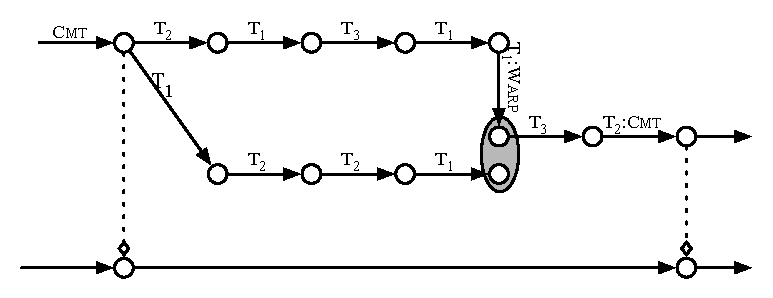
\includegraphics[width=3.2in]{simulation.eps}

\newcommand\obseq{\stackrel{\sim}{=}}
\newcommand\CS{\{c,\sigma\}}
\newcommand\CpSp{\{c',\sigma'\}}
\newcommand\numCS[1]{\{c_{#1},\sigma_{#1}\}}


\begin{figure*}
\centering
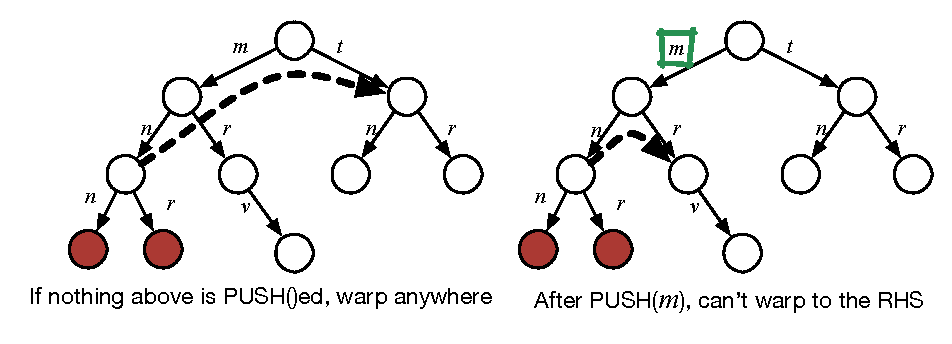
\includegraphics[width=5in]{stages.eps}
\caption{\red{caption.}}
\end{figure*}

\section{Technical Background}

In this section we describe a generic language of transactions and
define an idealized semantics for concurrent transactions called the
atomic semantics, in which there are no interleaved effects on the
shared state. 
%
The model preliminaries generalize those provided previously~\cite{PMPY}.
%
We also define a notion of \emph{good} configurations
and in the next section we will define how one can warp from a 
configuraiton that is not good to one that is.

\paragraph{Operations and States.}
We assume a set $M$ of method calls or operations (\eg\
  \texttt{ht.put('a',5)}).
%
State is represented in terms of
logs of operation records. An operation record (or, simply, an ``operation'')
$
    \op = \langle \opname, \lstack_1, \lstack_2, \opid \rangle
$
is a tuple consisting of the operation name $m$, 
a thread-local pre-stack $\lstack_1$ (method arguments),
a thread-local post-stack $\lstack_2$ (method return values),
and a unique identifier $\opid$.
%
We assume a predicate $\fresh{\opid}$ that holds provided that $\opid$
is globally unique (details omitted for lack of space).
%
In the atomic semantics defined below, the shared state $\OPL :
\textsf{list } \op$ is an ordered list of operations.
%
We use notations such as $\OPL_1\cdot\OPL_2$ and $\OPL\cdot \op$ to
mean append and appending a singleton, resp.

%\begin{parameter}[From logs to states: $\allowedt{}$] 
We require a prefix-closed predicate on operation lists $\allowed{\OPL}$
that indicates whether an operation log $\OPL$ corresponds to a state.
% The sequential specification
%   is a predicate on operation lists: $\allowed{\OPL}$. We require that it
%   be prefix closed.
%\end{parameter}
%
%\noindent
For convenience we will also write $\OPL \allows \langle m, \lstack_1,
\lstack_2, \opid\rangle$ which simply means 
$\allowed{\OPL \cdot \langle m, \lstack_1,\lstack_2, \opid\rangle}$.
%
For example, if we have a simple TM
based on memory read/write operations we expect
$\;\;\allowed{\OPL\cdot \langle \texttt{a := x}, [x \mapsto 5], [x
  \mapsto 5, a \mapsto 5], \opid\rangle}$,
but 
$\;\;\neg \allowed{\OPL\cdot \langle \texttt{a := x}, [x \mapsto 5], [x
  \mapsto 5, a \mapsto 3], \opid\rangle}$ or more elaborate
specifications that involve multiple tasks.
%
Ultimately, we expect the $\allowed{}$ predicate to be induced by the
implementation's operations on the state, $\llbracket op\rrbracket :
\mathcal{P}(\mathsf{State} \times \mathsf{State})$, and initial
states $I$. 
% If we give a denotation to logs as $\llbracket \OPL \cdot op
% \rrbracket \equiv \llbracket \OPL \rrbracket ; \llbracket op
% \rrbracket$, and $\llbracket \epsilon \rrbracket \equiv I$ , where $
% S ; R \equiv \{ s' \mid \exists s \in S. (s,s') \in R \}$. Then we
% can define $\allowed{\OPL}$ simply by checking if the denotation is
% non-empty, $(\llbracket \OPL \rrbracket \neq \emptyset)$.

%\paragraph{Operational equivalence.}
We define a precongruence over operation logs $\OPL_1 \opeq \OPL_2$
coinductively, by requiring that all \allowedt\ extensions of the log $\OPL_1$, are also \allowedt\ extension to the log $\OPL_2$. 
% This definition will ultimately be used in the simulation between
% \PMPY{} and an atomic machine.
We use a coinductive definition so that the precongruence can be
defined up to all infinite suffixes.
%\begin{definition}[Shared log precongruence $\opeq$] For all $\OPL_1, \OPL_2$,
$$
\infer={\OPL_1 \opeq \OPL_2} 
%   {\deduce{\allowed{\OPL_1}}  {\allowed{\OPL_2}}
   {  \allowed{\OPL_1} \Rightarrow \allowed{\OPL_2}
     & \forall \op.\   (\OPL_1 \cdot \op) \opeq (\OPL_2 \cdot \op)}
$$
We use a double-line here to indicate greatest fixpoint.
%\end{definition}
%
Informally, the above definition says that 
there is no sequence of observations we can make of $\OPL_2$, that we can't also make of $\OPL_1$. 
This is more general than just considering the set of states reached from executing the first log is included in the second:
unobservable state differences are also permitted. 


\paragraph{Language.}

Threads execute code $c$ from some programming language that
includes thread forking, transactions $\tx{c}$,
method names such as $m$, and a \skipt\ statement. As done
elsewhere~\cite{pmpy}, we abstract away the programming
  language with a few semantic functions: \red{update this with pldi
    camera ready}
%
\begin{description}
\item[$\step{c}{m}{c'}$:] Within a transaction, code $c$ can be reduced to the pair
  $(m,c')$.  That is, $m$ is a next reachable method call in the
  reduction of $c$, with remaining code $c'$.

\item[$\tstep{c}{t}{c'}$:] Outside of a transaction, code $c$ can be reduced to the pair
  $(t,c')$.  Here $c'$ is the remaining code, and $t$ is either
  a local state update, or a transaction or a thread fork.

\item[$\nothing{c}$:] This predicate is true provided that there is a
  reduction of $c$ to $\skipt$ that does not encounter a method call.
\end{description}
%
These functions allow us to obtain a simple semantics, despite an
expressive input language, by introducing functions to resolve
nondeterminism between method operation names and at the end of a
transaction.
%  As an example, one might use the generic language:
% \[ \begin{array}{rcl}
%   c &::=& c_1\plust c_2 \MOR c_1 \semit c_2
%       \MOR (c)^* \MOR \skipt \MOR \tx{c} \MOR \opname
% \end{array} \]
% %
% which consists of nondeterministic choice, sequential
% composition, and nondeterministic looping.
%
We assume that code is well-formed in that a single operation name $\opname$ 
is always contained within a transaction. 


The atomic semantics $\xrightarrow{a}$,
in which transactions are executed instantly, without interruption
from concurrent threads is given in Appendix~\ref{apx:atomic}.
Threads in the atomic semantics are represented as a pair
$(c,\sigma)$ of the code $c$ and a small amount of local
information $\sigma$ used to model arguments and return values.


%%% Local Variables:
%%% mode: latex
%%% TeX-master: "paper"
%%% End:


\newcommand\obseq{\stackrel{\sim}{=}}
\newcommand\CS{\{c,\sigma\}}
\newcommand\CpSp{\{c',\sigma'\}}
\newcommand\numCS[1]{\{c_{#1},\sigma_{#1}\}}

%\newcommand\cred[3]{#1 \dashrightarrow (#2,#3)}
\newcommand\tstep[3]{#1 \lightning (#2,#3)}
\newcommand\stept{\lightning\!\lightning}
\renewcommand\step[3]{#1 \stept (#2,#3)}

\newcommand\BigStep{\Downarrow}


\section{Preliminaries}

In this section we describe a generic language of transactions and
define an idealized semantics for concurrent transactions called the
atomic semantics, in which there are no interleaved effects on the
shared state. 
%
The model preliminaries generalize those provided previously~\cite{PMPY}.
%
We also define a notion of \emph{good} configurations
and in the next section we will define how one can warp from a 
configuraiton that is not good to one that is.

\paragraph{Language.}
%
We assume a set $M$ of method calls (\eg\
  \texttt{ht.put('a',5)}).
Threads execute code $c$ from some programming language that
includes thread forking, transactions $\tx{c}$,
method names such as $m$, and a \skipt\ statement.
Our first trick is to abstract away the programming
  language with a few functions:
%
\begin{description}
\item[$\step{c}{m}{c'}$:] Within a transaction, code $c$ can be reduced to the pair
  $(m,c')$.  That is, $m$ is a next reachable method call in the
  reduction of $c$, with remaining code $c'$.

\item[$\tstep{c}{t}{c'}$:] Outside of a transaction, code $c$ can be reduced to the pair
  $(t,c')$.  Here $c'$ is the remaining code, and $t$ is either
  a local state update, or a transaction or a thread fork.

\item[$\nothing{c}$:] This predicate is true provided that there is a
  reduction of $c$ to $\skipt$ that does not encounter a method call.
\end{description}
%
These functions allow us to obtain a simple semantics, despite an
expressive input language, by introducing functions to resolve
nondeterminism between method operation names and at the end of a
transaction. As an example, one might use the generic language:
\[ \begin{array}{rcl}
  c &::=& c_1\plust c_2 \MOR c_1 \semit c_2
      \MOR (c)^* \MOR \skipt \MOR \tx{c} \MOR \opname
\end{array} \]
%
which consists of nondeterministic choice, sequential
composition, and nondeterministic looping.
%
We assume that code is well-formed in that a single operation name $\opname$ 
is always contained within a transaction. 

\paragraph{Operations and logs.}
%
State is represented in terms of
logs of operation records. An operation record (or, simply, an ``operation'')
$
    \op = \langle \opname, \lstack_1, \lstack_2, \opid \rangle
$
is a tuple consisting of the operation name $m$, 
a thread-local pre-stack $\lstack_1$ (method arguments),
a thread-local post-stack $\lstack_2$ (method return values),
and a unique identifier $\opid$.
%
We assume a predicate $\fresh{\opid}$ that holds provided that $\opid$
is globally unique (details omitted for lack of space).
%
In the atomic semantics defined below, the shared state $\OPL :
\textsf{list } \op$ is an ordered list of operations.
%
We use notations such as $\OPL_1\cdot\OPL_2$ and $\OPL\cdot \op$ to
mean append and appending a singleton, resp.

\begin{parameter}[From logs to states: $\allowedt{}$] 
We require a prefix-closed predicate on operation lists $\allowed{\OPL}$
that indicates whether an operation log $\OPL$ corresponds to a state.
% The sequential specification
%   is a predicate on operation lists: $\allowed{\OPL}$. We require that it
%   be prefix closed.
\end{parameter}

\noindent
For convenience we will also write $\OPL \allows \langle m, \lstack_1,
\lstack_2, \opid\rangle$ which simply means 
$\allowed{\OPL \cdot \langle m, \lstack_1,\lstack_2, \opid\rangle}$.
%
For example, if we have a simple TM
based on memory read/write operations we expect
$\;\;\allowed{\OPL\cdot \langle \texttt{a := x}, [x \mapsto 5], [x
  \mapsto 5, a \mapsto 5], \opid\rangle}$,
but 
$\;\;\neg \allowed{\OPL\cdot \langle \texttt{a := x}, [x \mapsto 5], [x
  \mapsto 5, a \mapsto 3], \opid\rangle}$ or more elaborate
specifications that involve multiple tasks.
%
Ultimately, we expect the $\allowed{}$ predicate to be induced by the
implementation's operations on the state, $\llbracket op\rrbracket :
\mathcal{P}(\mathsf{State} \times \mathsf{State})$, and the initial
states, $I$. 
% If we give a denotation to logs as $\llbracket \OPL \cdot op
% \rrbracket \equiv \llbracket \OPL \rrbracket ; \llbracket op
% \rrbracket$, and $\llbracket \epsilon \rrbracket \equiv I$ , where $
% S ; R \equiv \{ s' \mid \exists s \in S. (s,s') \in R \}$. Then we
% can define $\allowed{\OPL}$ simply by checking if the denotation is
% non-empty, $(\llbracket \OPL \rrbracket \neq \emptyset)$.

\paragraph{Operational equivalence.}
We define a precongruence over operation logs $\OPL_1 \opeq \OPL_2$
coinductively, by requiring that all \allowedt\ extensions of the log $\OPL_1$, are also \allowedt\ extension to the log $\OPL_2$. 
% This definition will ultimately be used in the simulation between
% \PMPY{} and an atomic machine.
We use a coinductive definition so that the precongruence can be
defined up to all infinite suffixes.

\begin{definition}[Shared log precongruence $\opeq$] For all $\OPL_1, \OPL_2$,
$$
\infer={\OPL_1 \opeq \OPL_2} 
%   {\deduce{\allowed{\OPL_1}}  {\allowed{\OPL_2}}
   {  \allowed{\OPL_1} \Rightarrow \allowed{\OPL_2}
     & \forall \op.\   (\OPL_1 \cdot \op) \opeq (\OPL_2 \cdot \op)}
$$
We use a double-line here to indicate greatest fixpoint.
\end{definition}

\noindent
Informally, the above definition says that 
there is no sequence of observations we can make of $\OPL_2$, that we can't also make of $\OPL_1$. 
This is more general than just considering the set of states reached from executing the first log is included in the second:
unobservable state differences are also permitted. 



\newcommand\myT{T}
\newcommand\fork[1]{\texttt{fork }#1}
\newcommand\local[1]{\texttt{local }#1}
\newcommand\txnstep[1]{\;\underrightharpdown{\;#1\;}\;}
\newcommand\txnstept[1]{\underrightharpdown{\;#1\;}}

\subsection{Unconstrained Transition System}

We now defined a generic transition system in which threads may
interleave their effects however they please. Clearly, this transition
system is not serializable.

\figbox{\footnotesize
{\bf Unconstrained Machine Rules} $\xrightarrow{}$
$$
\infer[\text{\sc AFin}]{ 
  \As_1 \cdot (c,\sigma) \cdot \As_2, G  \xrightarrow{a}
  \As_1 \cdot \As_2, G 
}{
  \nothing{c}
}
$$
$$
\infer[\text{\sc AFork}]{ 
  \As_1 \cdot (c,\sigma) \cdot \As_2, G  \xrightarrow{a}
  \As_1 \cdot (c_2,\sigma) \cdot (c',\sigma) \cdot \As_2, G 
}{
  \tstep{c_1}{\fork{c}}{c_2}
}
$$
$$
\infer[\text{\sc ALocal}]{ 
  \As_1 \cdot (c,\sigma) \cdot \As_2, G  \xrightarrow{a}
  \As_1 \cdot (c',\sigma') \cdot \As_2, G 
}{
  \tstep{c}{\local{R}}{c'} & R\ \sigma\ \sigma'
}
$$
$$
\infer[\text{\sc ATxn}]{ 
  \As_1 \cdot (c_1,\sigma) \cdot \As_2, G  \xrightarrow{a}
  \As_1 \cdot (c_2,\sigma') \cdot \As_2, G'
}{
  \red{\text{fix this rule}} & 
  \step{c}{m}{c_2} &
  \tstep{c_1}{\tx{c'}}{c_2} &
  \OPL_1 \allows \langle m,\sigma,\sigma' \rangle &
  (c',\sigma),G \BigStep \sigma',G'
}
$$
}




\subsection{Serializable Transition System}


\paragraph{Atomic transition system}.
We define a simple atomic semantics, given in Figure~\ref{fig:atomic}
in which transactions are executed instantly, without interruption
from concurrent threads. The semantics is a relation
$\xrightarrow{a}$ over pairs consisting of a list of concurrent
threads $\As$ and a shared state $\OPL$. 
A single thread $(c,\sigma)\in\As$ is a code $c$ and local state $\sigma$. 
% The relation $\xrightarrow{a}^{*}$ is reflexive,
% transitive, and permits a thread to complete (rules
% {\sc ams\_refl}, {\sc ams\_trans}, {\sc ams\_end}, respectively).

We begin with Figure~\ref{fig:atomic}(b).
%
The atomic machine can take an {\sc AFin} step when there is a thread
$(c,\sigma)$ that can complete, \ie~$\nothing{c}$.
%
The {\sc AFork} rule allows a new thread
$(c',\sigma)$ to be forked from thread $(c,\sigma)$.
%
The {\sc ALocal} rule involves manipulating the thread-local state
$\sigma$ to $\sigma'$.
%
Finally, the {\sc ATxn} rule says that if thread executing code $c_1$ can reduce to a 
transaction $\tx{c'}$, then the transaction $c'$ is executed
atomically by the big step rules $\BigStep$ described next.

Figure~\ref{fig:atomic}(a) illustrates the
big step semantics $\BigStep$, which uses $\stept$ and $\nothing{}$ 
(rules {\sc BSStep} and {\sc BSFin}, respectively). These rules
scan through the nondeterminism in $\tx{c}$ to find a next operation
name $m$ or a path to $\skipt$ denoting the end of the transaction.
%
{\sc BSStep} can be taken provided that the operation $\langle m,\sigma,\sigma'\rangle$ is
permitted and that $(c_2,\sigma')$ can be
entirely reduced to $(\sigma'',\OPL_2)$.
%  Note that there a new operation identifier $\opid_1$
% is introduced. We require $\opid_1$ to be globally unique
% (formalization of \textsf{fresh} is omitted for lack of space).

%\red{explain bsstep. we go from $\OPL_1$ to $\OPL_2$ .... bsfin
%  basically copies the $\OPL$ from left of $\Downarrow$ to the right}








\begin{figure}
\figbox{\footnotesize
(a) {\bf Atomic Machine Big Step Transaction Rules} $\BigStep$
$$
\infer[\text{\sc BSFin}]{
  (c,\sigma),\OPL \BigStep c,\OPL
}{\nothing{c}}
\qquad
\infer[\text{\sc BSStep}]{
  (c,\sigma),\OPL_1 \BigStep \sigma'',\OPL_2
}{
  \deduce{
    (c_2,\sigma'),
    \OPL\cdot[\langle m,\sigma,\sigma' \rangle]
   \BigStep \sigma'',\OPL_2
 }{
   \deduce{\OPL_1 \allows \langle m,\sigma,\sigma' \rangle}
   {\step{c}{m}{c_2}}
 }
}
$$
(b) {\bf Atomic Machine Rules} $\xrightarrow{a}$
$$
\infer[\text{\sc AFin}]{ 
  \As_1 \cdot (c,\sigma) \cdot \As_2, G  \xrightarrow{a}
  \As_1 \cdot \As_2, G 
}{
  \nothing{c}
}
$$
$$
\infer[\text{\sc AFork}]{ 
  \As_1 \cdot (c,\sigma) \cdot \As_2, G  \xrightarrow{a}
  \As_1 \cdot (c_2,\sigma) \cdot (c',\sigma) \cdot \As_2, G 
}{
  \tstep{c_1}{\fork{c}}{c_2}
}
$$
$$
\infer[\text{\sc ALocal}]{ 
  \As_1 \cdot (c,\sigma) \cdot \As_2, G  \xrightarrow{a}
  \As_1 \cdot (c',\sigma') \cdot \As_2, G 
}{
  \tstep{c}{\local{R}}{c'} & R\ \sigma\ \sigma'
}
$$
$$
\infer[\text{\sc ATxn}]{ 
  \As_1 \cdot (c_1,\sigma) \cdot \As_2, G  \xrightarrow{a}
  \As_1 \cdot (c_2,\sigma') \cdot \As_2, G'
}{
  \tstep{c_1}{\tx{c'}}{c_2} &
  (c',\sigma),G \BigStep \sigma',G'
}
$$
}
\caption{\label{fig:atomic} Atomic semantics of concurrent threads.}
\end{figure}


\begin{definition}[Serializable transition system]
For all $\Ts,\OPL$, we say that a fragment 
$\xrightarrow{ser}$ of transition system $\xrightarrow{}$ is
serializable provided that 
$\xrightarrow{ser}$ simulates $\xrightarrow{a}$.
\end{definition}

As previously shown, the Push/Pull transition system is such a
serializable transition system~\cite{PMPY}.

\begin{definition}[Good configuration]
A configuration $\Ts,\OPL$ is \emph{good} provided that it is reachable in
some serializable transition system $\xrightarrow{ser}$
\end{definition}



%%%%%%%%%%%%%%%%%%%%%%%%%%%%%%%%%%%%%%%%%%%%%%%%%%%%%%%



\section{Trace Warping}

The idea of trace warping is to, at some point of execution, jump to
an alternate trace that is consistent what what we have observed so
far. 

Formally, a ``warp'' from a configuration $\Ts,G$ to another
configuration $\hat{\Ts},\hat{G}$ can be thought of two steps:
\begin{enumerate}
\item Taking some $n$ steps to another warp configuration:
  $\Ts,G \xrightarrow{}^{*} \Ts',G'$
\item Swapping the shared log $G'$ with observationally equivalent
  $\hat{G}$. That is,  $\hat{G} \opeq G'$
\end{enumerate}

% $$
% \infer[\text{\sc warp}]{ \Ts, G \xrightarrow{\textsf{warp}} \hat{\Ts}, \hat{G} }
% {
%   \begin{array}{lll}    
%     \text{\underline{Local crit.}} &: \Ts,G \xrightarrow{}^{*} \Ts',G'\\
%     \text{\underline{Global crit.}} &: G' \opeq \hat{G} & \text{(implies \allowedt)}\\
%   \end{array}
% }
% $$

%    \forall `G.\ `G \text{ prefix of } G.\\
%    \text{\underline{Local crit.}} &: \forall \{\hat{c},\hat{\sigma},\hat{L}\} \in \hat{\Ts}.\  \lfloor  \hat{G} \rfloor_{\hat{t}} \sim L


%    \exists \hat{\OPL} = \numOP{1} \cdots \numOP{n}.\\
%\allowed{\hat{\OPL}} \\

In practice, there are many warp configurations that can be calculated
conveniently. For one, uncommitted transactions can rollback (dropping
their effects) and then some number of (intereleaved) steps can be taken.
%
It is often convenient to think of a \emph{reference point}, which is
a previously reached configuration $\Ts_0,G_0$ from which one might
compute subsequently reachable warp points $\hat{\Ts},\hat{\OPL}$.


%\item jump each thread $\CSL\in \Ts$ to $\CpSpLp\in\hat{\Ts}$ such that:\\
%    $c' = c$ (could relax this in the future)\\
    
\begin{theorem}[Serializability]
Corollary to the serializability of the Push/Pull model~\cite{pmpy}.
\end{theorem}


\paragraph{Discussion}

This section carves out a large space of possibilities for where one
might warp to. Some things to consider:

\begin{itemize}
\item Pessimistic/Optimistic destinations 
  (our implementation does Pessimistic)
\item Serial-vs-Serializable destinations
  (our implementation does Serial).\\
  For serializabile, the criteria of {\sc push} and {\sc pull} give
  sufficient conditions in terms of left/right-movers.
\end{itemize}



%%% Local Variables: 
%%% mode: latex
%%% TeX-master: "paper"
%%% End: 


\input{formal}

\begin{figure}[t]
\begin{center}
\begin{tabular}{l}
\statement{s ::= m.put(k, v)}\\
\hspace{15pt} \statement{|\ x=m.get(k)}\\
\hspace{15pt} \statement{|\ m.remove(k)}\\
\hspace{15pt} \statement{|\ x=m.putIfAbsent(k, v, v')}\\
\statement{c ::= x==NULL\ |\ x!=NULL}\\
\end{tabular}
\end{center}
\caption{Statements and conditions}
\label{fig:language}
\end{figure}

\section{Language}
We will formalize our concrete and abstract semantics on the language in Fig. \ref{fig:language}. We distinguish between statements in \statement{s} and Boolean conditions in \statement{c}. Formally, $\statements = \statement{s} \cup \statement{c}$. We assume that all statements are atomic.

We represent transactions through control flow graphs (CFGs). Let $\labels$ the set of program labels. We suppose that $\statement{entry}, \statement{exit} \in \labels$ represents the entry and the exit label, respectively. A CFG is represented by a graph $\cfg = (\labels \times \edges)$ where the set of edges $\edges=(\labels \times \labels \times \statements)$ connects two vertexes in $\labels$ with a label that may be a statement in \statement{s} (to represent a sequential step) or \statement{c} (to represent a conditional jump). Therefore, each node in the CFG may have (i) one out edge with a label in \statement{s}, or (ii) two out edges with labels in \statement{c}.

A program \statement{p} is made by a (finite) set of transactions, and each transaction is represented by a cfg. Therefore, we represent a program made by $n$ transactions by a tuple of $n$ cfgs (where the $i$-th element represents transaction $i$). Formally, $\statement{p} \in \cfg^n$.

\todo{Should we discuss that the number of edges is between $|\labels|$ and $2*|\labels|$. This would be helpful to discuss the complexity of our approach}

\todo{Add running example}


\section{Concrete domain and semantics}
Our concrete domain is a standard finite trace domain. We define by $\trace{\cset{A}}$ the set of all finite traces of elements in $\cset{A}$.


Let $\cstatesmemory$ be the set of concrete states that represent both the shared and the internal memory state of the system. We suppose that an atomic small-step semantics $\to : \funzione{\cstatesmemory \times \statements}{\cstatesmemory}$ is provided. Given $n$ transactions, the definition of our concrete trace semantics relies on labeled states $\Sigma = \labels^n \times \cstatesmemory$.
Based on this semantics, we define the program semantics as follows:

\[
\begin{array}{l}
\csemantics{S}{\statement{p}, \sigma_0} = \textit{lfp}_{(\cel{L}_0, \cel{\sigma}_0)}^{\subseteq} \lambda \cset{T} . \cset{T} \cup\\
\left\{
\begin{array}{l}
 \{(\cel{L}_0, \cel{\sigma}_0) \to \cdots \to (\cel{L}_{i-1}, \cel{\sigma}_{i-1}) \to (\cel{L}_i, \cel{\sigma}_i) :\\
\hspace{10pt} (\cel{L}_0, \cel{\sigma}_0) \to \cdots \to (\cel{L}_{i-1}, \cel{\sigma}_{i-1})  \in \cset{T} \land\\
\hspace{10pt} \statement{t} \in \dom{\statement{p}} \land \exists \cel{l} \in \labels, \statement{st} \in \statements : (\pi_{\statement{t}}(\cel{L}_{i-1}), \cel{l}, \statement{st}) \in \pi_2(\statement{p}(\statement{t})) \land\\
\hspace{10pt}\cel{L}_i = \replace{\cel{L}_{i-1}}{\statement{t}}{\cel{l}} \land (\cel{\sigma}_{i-1}, \statement{st}) \to \cel{\sigma}_{i}
\end{array}
\right\}\\
\end{array}
\]
where $\cel{L}_0=\statement{entry}^{|\dom{\statement{p}}|}$ and $\replace{\cel{t}}{i}{v}$ replaces the $i$-th component of the tuple $\cel{t}$ with value $v$.

\subsection{Property}

We distinguish between \emph{good} and \emph{bad} executions by looking to the interleaving of the execution of different transactions \todo{Probably we should add something about the state (e.g., to check that two statements interfer on the same key). This is just an abstraction of the trace.}.


An action performed by a transaction $i$ on a key $\statement{k}$ is represented by $a_i(\statement{k}) \in \actions$. We distinguish between read and write actions represented by $r$ and $w$, respectively. Statements in \statement{s} by transaction $i$ are interpreted as read and/or write as follows:
\begin{itemize}
\item \statement{m.put(k, v)} is represented by $w^i(\statement{k})$,
\item \statement{x=m.get(k)} is represented by $r^i(\statement{k})$,
\item \statement{m.remove(k)} is represented by $w^i(\statement{k})$, and
\item \statement{x=m.putIfAbsent(k, v, v')} is represented by $r^i(\statement{k})$ (if \statement{k} is already in the map) \emph{and} $w^i(\statement{k})$ (otherwise).
\end{itemize}
Given a statement $\statement{st}$ and a transaction $k$, we define by $\getaction{\statement{st}}{k}$ the function that returns the corresponding action.

We then define a function $\projectTrace{\statement{p}, \tau}$ that projects a trace of states $\tau$ produced by a program \statement{p} to the sequence of actions it performed\footnote{In the formal definition we ignore execution steps that do not produce actions (i.e., the execution of statements in \statement{c})}:

\[
\begin{array}{l}
\projectTrace{\statement{p}, (\cel{L}_0, \cel{\sigma}_0) \to \cdots \to (\cel{L}_n, \cel{\sigma}_n)} = \{
\cel{a}_1 \to \cdots \to \cel{a}_n :\\
\hspace{10pt} \forall j \in [1..n] : \extractstep{\statement{p}}{\cel{L}_{j-1}}{\cel{L}_j}=(\statement{t}, k) \land\\
\hspace{57pt} \getaction{\statement{t}}{k}=\cel{a}_j \}\\
\end{array}
\]
where $\extractstep{\statement{p}}{\cel{L}}{\cel{L}'}$ given two labels representing a step of the execution and the program returns the statement and the transaction that performed the step.

We need to build a function $\isBad{\cel{a}_1 \to \cdots \to \cel{a}_n}$ returns $\true$ if and only if the given sequence of actions represents a serializability violations.\todo{This is not quite right, revise it later}

Finally, given a program $\statement{p}$ and an initial state $\cel{\sigma}_0$, we can partition the set of traces into good and bad traces.

\[
\begin{array}{l}
\cset{T}=\csemantics{S}{\statement{p}, \sigma_0}\\
\badtraces = \{\tau \in \cset{T} : \isBad{\projectTrace{\tau}}\}\\
\goodtraces = \cset{T} \cap \badtraces\\
\end{array}
\]

%We suppose that the oracle is such that if something has happened, than all the traces from there on will be bad. This is formalized as follows:
%
%\[
%\begin{array}{c}
%\forall \sigma_0 \to \cdots \to \sigma_i \in \badtraces, \nexists \sigma_0 \to \cdots \to \sigma_i \to \sigma_{i+1} \to \cdots \to \sigma_j : \\
%\sigma_0 \to \cdots \to \sigma_i \to \sigma_{i+1} \to \cdots \to \sigma_j \notin \badtraces 
%\end{array}
%\]
%
%\todo{We can reformulate this by removing the double negation and with universal quantification on the second trace - not sure what is easier to understand and for the formal proofs}


\subsection{Abstract domain and semantics}
As usual in abstract interpretation, we approximate the concrete domain and semantics with an abstract domain and semantics. The abstract domain forms a Galois connection with the concrete domain, while the abstract semantics approximates the concrete one. \todo{The abstract semantics should be tuned at the level of traces, so we can present the Cartesian product as an abstraction of the original traces}

\section{Warping system}


\subsection{Observational Equivalence}

We assume that observations on the state can only be made by state transformers. We denote
$\sigma \xrightarrow{m/k} \sigma'$ a state transition where some method $m$ has been invoked, and value $k$ returned (we leave the domains of $m$ and $k$ undefined for now).

For two states $\sigma_1$ and $\sigma_2$, observational equivalence is defined as follows:

$$\sigma_1 \sim \sigma_2 \;\;\Leftrightarrow\;\;
\begin{array}{l}
  \sigma_1 \xrightarrow{m/k_1} \sigma_1' \text{ implies that }\\
  \begin{array}{rl}
      (i)&\exists k_2\ \sigma_2'.\ \sigma_2  \xrightarrow{m/k_2} \sigma_2'\\
      (ii)&\forall k_2\ \sigma_2' \text{ such that } \sigma_2  \xrightarrow{m/k_2} \sigma_2'.\\
          & \sigma_2 \xrightarrow{m/k_2} \sigma_2' \;\wedge\; k_1 = k_2  
          \end{array}
\end{array}
$$

\subsection{Trace Warping}

\newcommand\warp{\textsf{warp}}
Consider some  bad trace $\tau = \sigma_0 \to \cdots \to \sigma_i$. We want to find a good trace $\tau' = \sigma'_0 \to \cdots \to \sigma'_j$ such that $\sigma_i \sim \sigma'_j$. We do this via a \emph{warp} function $f$, which adjusts the state of the bad execution to fall into the good execution. 

For $\tau = \sigma_0 \to \cdots \to \sigma_i \in \badtraces$, 
and $\tau' = \sigma'_0 \to \cdots \to \sigma'_j$,
$$
\warp(\sigma_i,f(\sigma_i))
\;\;\;\Leftrightarrow\;\;\;
f(\sigma_i) \sim \sigma_j'
\;\wedge\;
\sigma_0 \sim \sigma'_0
\;\wedge\;
\tau' \notin \badtraces
$$

\todo{consider not including $\badtraces$ in the def of warp. maybe easier to permit warping to other bad traces}


\subsection{Abstract Trace Warping}

\todo{define hat sim}

\newcommand\awarp{\textsf{awarp}} We now lift to the abstract domain.  Consider some bad trace $\tau = \hat{\sigma}_0 \to \cdots \to \hat{\sigma}_i$. We want to find a good trace $\tau' = \hat{\sigma}'_0 \to \cdots \to \hat{\sigma}'_j$ such that $\hat{\sigma}_i \hat{\sim} \hat{\sigma}'_j$. We do this via an \emph{abstract warp} function $\hat{f}$, which adjusts the state of the bad execution to fall into the good execution.

For $\tau = \hat{\sigma}_0 \to \cdots \to \hat{\sigma}_i \in \badtraces$, 
and $\tau' = \hat{\sigma}'_0 \to \cdots \to \hat{\sigma}'_j$,
$$
\warp(\hat{\sigma}_i,\hat{f}(\hat{\sigma}_i))
\;\;\;\Leftrightarrow\;\;\;
\hat{f}(\hat{\sigma}_i) \hat{\sim} \hat{\sigma}_j'
\;\wedge\;
\hat{\sigma}_0 \hat{\sim} \hat{\sigma}'_0
\;\wedge\;
\tau' \notin \badtraces
$$




\section{Cartesian product of transactions}
Given a tuple of $n$ transactions $\cset{T} \in \cfg^n$, we build up the Cartesian product of the cfg of these transactions. Formally, we define the cfg of $\cset{T}$ by $\cel{cfg}_{\cset{T}} = \square_{(\cel{L}_i, \cel{E}_{i}) \in \cset{T}} (\cel{L}_i, \cel{E}_{i})$ where $\square$ denotes the Cartesian product of graphs\todo{Cite something?}. Formally,
\[
\begin{array}{l}
\square_{(\cel{L}_i, \cel{E}_{i}) \in \cset{T}} (\cel{L}_i, \cel{E}_{i}) = (\cel{V}, \cel{E}) :\\
\hspace{20pt} \cel{V}=\Pi_{(\cel{L}_i, \cel{E}_{i}) \in \cset{T}} \cel{L}_i\\
\hspace{20pt} \cel{E}=
\left\{
\begin{array}{l}
(\cel{L}, \cel{L}', \statement{st}) : \cel{L}, \cel{L}' \in \cel{V} \land\\
\hspace{40pt} \exists j \in [1..n] : \forall i \in [1..n] \setminus \{j\}  : \cel{L}_i=\cel{L}'_i \land\\
\hspace{40pt} \exists (\cel{L}_j, \cel{L}'_j, \statement{st}) \in \cel{E}_j\\
\end{array}
\right\}
\end{array}
\]

The intuition behind the Cartesian product of cfgs is that (i) each node represents where the execution of each transaction is arrived, and (ii) each edge represents that one transaction performs the execution of an atomic step, while the others do not progress. In this way, we can rely on the Cartesian product of cfgs to compute the interleaving semantics.

\textbf{Put the running example here}

\subsection{Semantics}
On the Cartesian product of transactions we define the concrete semantics as follows:

\[
\begin{array}{l}
\csemantics{S_{CFG}}{\statement{cfg}_\statement{p}, \sigma_0} = \textit{lfp}_{(\cel{L}_0, \cel{\sigma}_0)}^{\subseteq} \lambda \cset{T} . \cset{T} \cup\\
\hspace{10pt} \left\{
\begin{array}{l}
\hspace{10pt} (\cel{L}_0, \cel{\sigma}_0) \to \cdots \to (\cel{L}_{i-1}, \cel{\sigma}_{i-1}) \to (\cel{L}_i, \cel{\sigma}_i) :\\
\hspace{10pt} (\cel{L}_0, \cel{\sigma}_0) \to \cdots \to (\cel{L}_{i-1}, \cel{\sigma}_{i-1})  \in \cset{T} \land\\
\hspace{10pt} \exists (\cel{L}_{i-1}, \cel{L}_i, \statement{st}) \in \pi_2(\statement{cfg}_\statement{p}) \land (\cel{\sigma}_{i-1}, \statement{st}) \to \cel{\sigma}_i\\
\end{array}
\right\}\\
\end{array}
\]



\begin{lemma}[Soundness of the concrete semantics on the Cartesian product of CFGs]
$\csemantics{S}{\cel{cfg}_{\cset{T}}, \sigma_0} \subseteq \csemantics{S_{CFG}}{\cel{cfg}_{\cset{T}}, \sigma_0}$
\end{lemma}

\todo{In theory, they are equal and we can prove it, but maybe this is not interesting, maybe yes - it depends if we need an underapproximation for the good traces}

\subsection{Bad flows}
Then we statically detect on the CFG of a set of transactions $\cel{cfg}_{\cset{T}}$ the flows that \emph{may} lead to bad executions. Therefore, we build up a data flow analysis that tracks what actions may reach each label in $\cel{cfg}_{\cset{T}}$.

In particular, we are only interested in triples made by these elements since the properties we want to check are on the last three actions \todo{We should enumerate the 4 cases and cite the work introducing them}. Therefore the abstract domain of our data-flow analysis is $(\labels \cup \{\epsilon\})^3$, where $\epsilon$ represents situation in which we have less than three elements. Our data flow analysis is forward and possible. Therefore, our analysis is defined by the following equations:

$$
\begin{array}{l}
\cfunction{In}(\cel{l}) = \bigcup_{(\cel{l'}, \cel{l}) \in \cel{e}} \cfunction{Out}(\cel{l'})\\
\cfunction{Out}(\cel{l}) = \cfunction{Gen}(\cel{l}) \setminus \cfunction{Kill}(\cel{l}) \\
\cfunction{Kill}(\cel{l}) = \{(\cel{a}_1, \cel{a}_2, \cel{a}_3) : (\cel{a}_1, \cel{a}_2, \cel{a}_3) \in \labels^3\}\\
\cfunction{Gen}(\cel{l}) = \{(\cel{a}_1, \cel{a}_2, \cel{a}_3) : \exists \cel{a}_4 \in \actions \cup \{\epsilon\}: (\cel{a}_2, \cel{a}_3, \cel{a}_4) \in \cfunction{In}(\cel{l}) \land\\
\hspace{125pt} \cel{a}_1 \in \getaction{\cfunction{getWeigth}(\cel{I})} \}
\end{array}
$$

where $\cel{e}$ represents the edges of the cfg, and $\getaction{\statement{st}}{TODO}$ returns the set of actions ($r$ and/or $w$) the given statement may perform.\todo{Since we have the statements of the edges and not in the nodes, the getLabel function is somewhat broken. I should add the out label and the transaction that performs the statement}

Finally, we tag the edges that could expose bad behaviors. For each edge 


In particular, for each edge in $\cel{cfg}_{\cset{T}}$ we consider all the triples of actions generated by this edge. If at least one of these triples represents a conflict, we tag the edge as bad.\todo{Note: we should have one triple per key, but since we are assuming to have only one key statically known we consider this case. This sounds weak}
Bad edges are aimed at over-approximating bad executions.

\begin{theorem}
$\forall \tau \in \badtraces \cap \csemantics{S}{\statement{p}, \sigma_0} : \tau \in \csemantics{S_C}{\cel{cfg}_{\cset{T}}, \sigma_0} \cap \badtraces$
\end{theorem}

\todo{We should define exactly the semantics over the cartesian product of cfgs and show how the trace is built from there}



\section{TVLA-based analysis}

We instantiated this framework with a TVLA based analysis. We adopted the following representation:
\begin{itemize}
\item we represent through a summary node what is inside the map at the beginning of the execution
\item for all the keys and the values that are parameters of the two transactions, we represent them with concrete nodes
\item we adopt a binary predicate $r$ to link the map to the summary node
\item we adopt a binary predicate $k$ to link a parameter key to the map to represent that the key is in the map (note that this predicate is always 0 or 1, never half!)
\item we adopt a binary predicate $val$ to represent that a key is connected to a value. This $val$ connects the summary node to itself to represent the initial values stored in the map, and it connects the concrete node of a parameter key to a concrete node of a parameter value if the key is insider the map and it is related to the given value
\end{itemize}

We then represent various entry state in which the predicate $k$ (and $val$ between parameter keys and parameters values) is 1 or 0 to represent all the possible combination when the entry map contains or not a parameter key (and the parameter key is related or not to a parameter value).

Given two abstract states of our analysis, we know that all their concretizations are observationally equivalent.

\begin{theorem}
$\forall \sigma_1, \sigma_2 \in \gamma({\ael{\sigma}}) : \sigma_1 \sim \sigma_2$
\end{theorem}


\section{Instance of the warping system}

Abstract domain $\astates^{\sharp} = \parts{\pair{\astates}{\{\mathtt{good}, \mathtt{bad}\}}}$

$\mathbb{Q}$ finite set of queries (with parameters)

This set of queries represents the set of observations we can make on a state of the execution (e.g., check if a key is in the map, get the value stored in a given key, ...). This means that we consider that two concrete states are observationally equivalent if they give the same answers to all these queries (Property 1).

First assumption: we have an $eval$ function (that evaluates a query) such that $\forall \statement{q} \in \mathbb{Q}, \ael{\sigma} \in \astates : \afunction{eval}(\statement{q}, \ael{\sigma}) \in \{\true, \false\}$. In particular, this means that we get precise answers to the queries (e.g., the key is / is not in a map), since we can answer only $\true$ or $\false$, and not $\top$. By Property 1 we have then that all the concrete states concretized from an abstract state $\ael{\sigma} \in \astates$ they belong to the same class. In fact, if we get as answer to a query on the abstract state $\true$ (or $\false$), we get $\true$ (or $\false$) on all the possible concretizations of $\ael{\sigma}$. 

Second assumption: we have a function $\Delta : \funzione{\pair{\astates}{\astates}}{\statements^*\cup \{\top\}}$. This function, given two states, returns the set of statements you have to execute to go from the first abstract state to the second one. Formally, $\asemantics{S}{\Delta(\ael{\sigma}, \ael{\sigma}'),\ael{\sigma}}=\ael{\sigma}'$ if $\Delta(\ael{\sigma}, \ael{\sigma}') \neq \top$.

Then we have an entry state made by good abstract states, we take the Cartesian product of the cfgs, and we compute entry and exit state per node in the cfg. We need to explain (1) how we assign good and bad, and (2) how we prove the correlation between entry and exit state preserving the concrete semantics.


%\pagebreak
%\onecolumn


\section{Preliminary Implementation}\label{Se:experiments}

We now report encouraging results of our preliminary implementation.
We have implemented the static analysis and the runtime synchronization algorithms, and performed an experimental evaluation over a set of four subjects taken from real-world code bases. 
\red{blend below withabove}
%\smartpar{Prototype System}
%\label{Se:system}
We have created a Java implementation of our static analysis for composed {\sf Map} operations, as described  in Section \ref{se:instance}. Given $n$ types of transactions, our implementation builds a serialized CFG as described in Section \ref{Se:concabs}, and then it computes a fixpoint over it relying on the abstract semantics formalized in Section \ref{sect:abstractsemantics}. We support all the operations listed in Section \ref{sect:language}. Static analysis running times are negligible compared to the rest of the process, and the analysis converges always in less than a second. Therefore, we do not report the running times of the static analysis.

As explained earlier, the interface with the runtime system is a relational corrective specification mapping prestates to sets of poststates that are obtainable via serializable execution of the transactions from the prestate. As a partial example, 
%\begin{center}
$[ {\sf k} \mapsto \bot , {\sf v} \mapsto v ] \leadsto \{ [ {\sf k} \mapsto v , {\sf v} \mapsto v ] \}$
%\end{center}
denotes that if we started from a prestate where ${\sf k}$ was not in the map and the value passed to the function was $v$, then in the poststate the key ${\sf k}$ is made to point to the value $v$ pointed-to by the second argument ${\sf v}$ in the prestate.
%
The runtime system $S$ is parameterized by the specification, which it loads at the beginning of the concurrent run. 

As discussed in Section \ref{sec:dynamicwarping}, in our current prototype all transactions are assumed to start simultaneously. This scenario is useful, for example, in loop parallelization. Each concrete transaction is mapped to its abstract counterpart, as explained in Section \ref{Se:concabs}. The mapping process also binds the concrete arguments of the transaction (i.e., the concrete object references) to their symbolic counterparts (e.g., the {\sf k} and {\sf v} symbols above). 

During execution, the runtime system monitors commit events. In our current prototype, we limit transactions to a single commit point before completion. Corrective synchronization occurs only on failed commits (as discussed in Section \ref{Se:guarantees}), in which case the transaction's shared log, local state and return value (if it exists) are all (potentially) modified according to the corrective specification. 

\OmerAdded{Analogously to the pruning technique used to map between states and their corrective counterparts, the decision whether a commit has failed is based on incremental pruning of the good global states $G$ according to the final states of committed transactions. If the final state of a transaction is not consistent with state $g \in G$, then $g$ is pruned out. If $G$ at any point becomes empty, then the system has reached a bad state.}

\smartpar{Summary of Subjects and Experiments}
%
We conducted experiments running our implementation on four subjects, all of which
are taken from popular open-source code bases and have been used in past studies\cite{oopsla/ShachamBASVY11,issta/ShachamYGABSV14}. We considered workload size and
concurrency level, ranging from 2 to 23 threads, and summarizing over 10 runs.
%
In each case,we compared against (i) a pessimistic concrete-level variant of STM, as available via version 1.3 of the Deuce STM (the latest version)\footnote{
		\url{https://github.com/DeuceSTM/DeuceSTM}
}, and (ii)  a lock-based synchronization algorithm boosted with {\sf Map} semantics \cite{ppopp/HerlihyK08}, such that the locks are of the same grain as their corresponding abstract locks in boosted STM.
%
We ran our experiments on two Intel Xeon 2.90GHz (16 cores) CPUs with 132GB of RAM.

For lack of space, the detailed results of the experiments can be found in Appendix~\ref{Se:perf}, considering factors such as number of threads and size of the workload. Here we simply report aggregate performance results, averaging across all workloads and concurrency
\begin{wrapfigure}[10]{r}{0.50\textwidth}
\begin{tabular}{|l|c|c|c|c|}
\hline
  & \multicolumn{2}{c|}{STM} & \multicolumn{2}{c|}{corrective sync.} \\
					\cline{2-5} 
					& workload & conc. & workload & conc. \\
\hline
Tomcat	  	 &	1.5\%		&	3\% & 29\%		& 30\% \\			   
dyuproject	 & 	18\%		& 	24\%	    & 30\% &	29\%	\\
Flexive 		&	17\%	  &		14\%			& 29\% & 30\%	\\ 
Gridkit 		&	20\% 	&		16\%		& 32\% & 31\%	\\
\hline\hline	
{\bf average} & {\bf 14\%} 	&   {\bf 14\%}    & {\bf 30\%}   & {\bf 30\%} \\
\hline
\end{tabular}
%\end{center}
\end{wrapfigure}
levels, are summarized to the right.
For completeness, we also note the absolute running times, as min/max intervals in seconds, for the lock-based solution for the workload and concurrency configurations respectively: Tomcat -- [6,10], [7,12]; dyuproject -- [6,9], [7,11]; Flexive -- [6,10], [7,11]; and Gridkit -- [6,9], [7,11]. 
The numbers are encouraging, indicating improvement over both locks and STM. More careful engineering, beyond our current prototype implementation, is likely to make the improvement more significant.


%In Figure~\ref{fig:case2Iter}, the X axis is the number of transactions in each thread, Y axis is the running time (unit: milliseconds). We fix the number of threads as 8. Although the number of transactions changes, the ratio between the $lock/stm$ time and the $warp$ time remains around 5, i.e., the $warp$ version runs as  5X times as the $lock/stm$ versions. We interpret the results in the following ways. First, the $lock$ version essentially serialize all the transaction instances because they involve the same key. The $stm$ version also exhibits the  parallelism embarrassingly in this case: Many transaction instances unconditionally update the location of the key in the map, which conflict with the transaction instances that read the location and force them to rollback. The $stm$ and $lock$ versions have similar performance because they  both serialize the transaction instances. Second, the speedup of our approach over $lock/stm$ is fixed when the thread number is fixed, indicating that the speedup is subject to the number of threads. 
%
%
%
%In Figure~\ref{fig:case2Th}, the X axis is the number of threads, Y axis is the running time. We fix the number of transactions each thread runs as 100. The ratio between the $lock/stm$ time and the $warp$ increases when the number of threads increases. For example, the $lock/stm$ version takes around 2X time as the $warp$ with 2 threads, around 3X time with 4 threads, around 5X with 8 threads, and remain 5X with more than 8 threads. This observation confirms our previous conclusion that the speedup is subject to the the number of threads. In this case, we get the best the speedup with 8 threads, where 8 is also the number of the cores, indicating that we make full exploitation of the cores with 8 threads. The figure shows that our approach has the dramatically better thread scalability than existing approaches. Another interesting observation is, when there is a single thread, the stm version takes 164 ms, while both our version and the lock version takes 112 ms. The stm takes longer time because the Deuce implementation instruments the classes on  the fly when they are loaded, which consumes extra time. 
%
%
%Figure~\ref{fig:case3Iter}, Figure~\ref{fig:case4Iter} and Figure~\ref{fig:case4Iter} show the performance when the workload increases and follow the same setting as the test 2 shown in Figure~\ref{fig:case2Iter}. Similar to Figure~\ref{fig:case2Th}, Figure~\ref{fig:case3Th}, Figure~\ref{fig:case4Iter} and Figure~\ref{fig:case4Iter} show the performance when the number of threads increases. From the figures, we see the trend of the lock version and our version resemble case 2, but the stm version behaves quite differently. An interesting observation is, the time difference between the stm version and ours is almost a constant. This suggests that the stm version achieves the same parallelism degree as ours, while incurring some extra  overhead of class instrumentation. We inspected the code and confirmed this conclusion. In these cases, many transaction instances first check and then update conditionally. After the first instances update, the following instances will fail the checking and are degenerated to read-only transactions. The read-only transactions allow the maximal parallelism like ours. 
%
%\subsection{Discussion}
%
%{\bf Execution Summary\ } The static analysis phase computes a set of execution summaries, each representing a legal execution, which are used as the input of the dynamic analysis phase.
%Each execution summary describes (i) the return value of each transaction instance and (ii) the final map state
% 
%
%In our experiments,  we have two threads running two types of transactions ($TX_1$ and $TX_2$) respectively. One exemplary execution summary is, $[key\rightarrow v^1_1, r^1_1:v^1_1, r^n_1:v^1_1, r^1_2:v^1_1, r^n_2:v^1_1]$, where $r^1_1$ is the symbolic form of the return value of $TX^1_1$ (1$st$ instance of $TX_1$), $v^1_1$ is the symbolic form of the value put by the transaction instance, and $r^1_1:v^1_1$ describes the return value of the transaction instance. The readers may notice $r^n_1$. This symbol represents the return value of the instances that are not explicitly specified.  Here $n$ is determined by the capability of the static analysis. At runtime, we track the instance order and use $n$ by default if the number is not specified in the summary. The tracking of the instance order requires us to synchronize the first $n-1$ instances. However, the $n$ is typically a small number, and the synchronization overhead is negligible. We do not need to synchronize starting from the $n$th instance because all these instances are represented as $n$ by default. In addition, $key\rightarrow v^1_1$ tells what the key is associated with in the final map state. 
%
%The execution summary is not limited to the above basic case. In general, it is initial-state sensitive, schedule-oblivious and site-sensitive. 
%First, the initial state about whether the key is mapped to some value affects the computation of the execution summaries. Therefore, we prefix each execution summary with a specific initial state, e.g., the state with initial key $[key^{init}\rightarrow v^{init}]$ or the state without initial key $[key^{init}\rightarrow void]$.
%Second, our execution summary is designed to be oblivious of the schedules. The schedule-obliviousness frees us from tracking the schedules at runtime and avoids the high tracking overhead. Third, the execution summary is site-sensitive. A transaction $TX^1_1$ may put a value dynamically created at site $A$ to the map. We symbolically represent the value using the site and the occurrence of the site (inside the transaction instance), e.g., $A1$ in $TX^1_1$. The extent to which we can distinguish the occurrences is determined by the static analysis, e.g., how many iterations can be unrolled.
%
%
%{\bf Runtime System\ }
%The runtime works as follows. We first use the counters to track the transaction instance and assemble the symbolic return accordingly, e.g., $r^1_1$.
%Then we search for the symbolic value in the execution summaries, e.g., $v^1_1$. Last, using the symbolic value as a key, we look up the cache, which is maintained to associate each symbolic value with a runtime value, for the concrete runtime value.
%
%The second step, i.e., searching for symbolic value in the summaries, is challenging. The searching is demanded on the fly at the return of each transaction instance. 
%However, the returns should be consistent with each other such that the warped execution represents a realistic execution. In the other words, the return values should be searched for in the same execution summary. To achieve this, we implement an on-the-fly pruning algorithm. At the first return, it finds the symbolic value in a randomly picked execution summary. After the value is picked, the execution summaries with different value for the return will be pruned, leading to a smaller solution space. 
%The algorithm is iteratively applied. In addition, to achieve initial-state sensitivity, we also reduce the solution space based on the initial states. 
%
%Another tricky issue is, at some return, the symbolic value found in the execution summaries may have not been associated with any concrete runtime value yet.
%For example, at the return of $TX^1_2$, we find the returned value as $v^1_1$ but $TX^1_1$ has not been executed, then we cannot find the runtime value associated with $v^1_1$ in the cache. This case happens because the execution summary is computed for certain schedule, which differs from the current schedule. In this case, we apply the notify/wait primitives to synchronize the cache lookup and cache maintenance. Even more complex, the returned value may never be put into the cache if the value creation site is disabled in the current schedule, e.g., its guarding branch condition is false. We simply remove all the guarding branches for the creation site such that it is always executed. This simple strategy is based on the insight that we treat the transaction as a blackbox and we only care about its return values. It is unnecessary to preserve the internal program semantics.
%
%
%We also implemented the optimization for the caching. From the summaries, we see that only the values put by the first few transactions are used. Therefore, we only record such values into the cache and discard the rest at runtime.
%
%
%
%
%
%
%\subsection{Evaluation}
%
%%TODO: check if we need to remove teh business op from the warp version.
%For performance measurement, we compare 4 versions with different types of synchronizations, the original version $orig$, the abstract key locking version $key$, the software transactional memory version $stm$, and the warping version $warp$.  The original version is without any synchronization, which may produce incorrect outputs. 
%We use this version to approximate the best performance any synchronization can achieve. The abstract key locking protects each key with a unique lock~\cite{}. As compared to protecting the whole map with a single lock, it allows parallelism among the invocations with different keys. For the software transactional memory, we use the open sourced implementation {\sf Deuce}~\cite{}. {\sf Deuce} features the easiness of use. {\sf Deuce} is essentially a Java agent that instruments the classes during the class loading to insert the STM functionality. However, the JDK classes are loaded before the agent starts to work. Therefore, we re-import the JDK implementation as application classes, which {\sf Deuce} successfully apply to. 
%The $warp$ version adopts our algorithm. In our evaluation, we use both the initial state with the key and the initial state without the key.  For space reason and clarity of figure, we only show the result based on the initial state with the key (other results are put into the technique report).
%
%
%Our benchmark is adapted from real world applications, including XXX and YYY. In our experiment, we consider two types of transactions for each benchmark, and each thread runs a combination of the transactions. In our experiment, we measure the performance under two changes: (1) We fix the number of threads as 8, the number of cores in the machine, and then change the number of transactions each thread runs from 10 to 100. This setting helps us understand the performance in different workloads, (2) we fix the number of transactions each thread runs as 100, and change the number of threads following the sequence: 1,2,4,6,8,10,12,14,16. This setting allows us to study the thread scalability. In our experiments, all threads operate on the same key.

%\begin{figure*}
%\centering
%\subfloat[{Case 2 with the increasing workload}]{\label{fig:case2Iter}\includegraphics[width=0.33\textwidth]{../../eval/case2-varyIter.pdf}}
%\subfloat[{Case 2 with the increasing number of threads}]{\label{fig:case2Th}\includegraphics[width=0.33\textwidth]{../../eval/case2-varyThreads.pdf}}
%\\
%\subfloat[{Case 3 with the increasing workload}]{\label{fig:case3Iter}\includegraphics[width=0.33\textwidth]{../../eval/case3-varyIter.pdf}}
%\subfloat[{Case 3 with the increasing number of threads}]{\label{fig:case3Th}\includegraphics[width=0.33\textwidth]{../../eval/case3-varyThreads.pdf}}
%\\
%\subfloat[{Case 4 with the increasing workload}]{\label{fig:case4Iter}\includegraphics[width=0.33\textwidth]{../../eval/case4-varyIter.pdf}}
%\subfloat[{Case 4 with the increasing number of threads}]{\label{fig:case4Th}\includegraphics[width=0.33\textwidth]{../../eval/case4-varyThreads.pdf}}
%\\
%\subfloat[{Case 5 with the increasing workload}]{\label{fig:case5Iter}\includegraphics[width=0.33\textwidth]{../../eval/case5-varyIter.pdf}}
%\subfloat[{Case 5 with the increasing number of threads}]{\label{fig:case5Th}\includegraphics[width=0.33\textwidth]{../../eval/case5-varyThreads.pdf}}
%\caption{Performance Measurement}
%\label{fig:perf}
%\vspace{-1em}
%\end{figure*}









\section{Related work}

To the best of our knowledge there have been no works that treat
synchronization of transactions from a principalled, corrective
manner. We now summarize other recent programming methodologies in
exploiting parallelism within transactional systems. These works
explore different ways to improve performance by either reducing
aborts and/or the extent to which a transaction rolls back. As a clear
indication of distinction, note that our corrective approach has no
notion of rollback.

Checkpointing in transactional boosting~\cite{spaa08a} and nested
transactions~\cite{ont,beeri} attempts to, in the event of a conflict,
avoid wasted work done by transactions by only partially
aborting. Elastic transations~\cite{FGG:DISC09} similarly avoid wasted
work by splitting into multiple pieces.  The Janus algorithm for lazy
optimistic synchronization~\cite{TMFS:PLDI12}, \red{does...}
Golan-Gueta \emph{et al.}~\cite{GRSY:PLDI13} on synchronization with
foresight \red{does...}  Tripp \emph{et al.}~\cite{TKS:OOPSLA13} show
how nondeterminism in data-structure specifications offers an
opportunity for increased parallelism.



Our work employs \emph{static analysis} to generate information that
can be used at runtime to improve performance. Some have explored
others ways of using static information, e.g., to infer locking
schemes for transactions~\cite{gulwani}.

Bill McCloskey's POPL'05/06 work
Peter Hawkins' works
Guy's work

%%% Local Variables:
%%% mode: latex
%%% TeX-master: "paper"
%%% End:


\section{Conclusion and Future Work}

We have presented an alternative to the lock- and retry-based synchronization methods, which we dub \emph{corrective}. The key insight is to correct a bad execution, rather than retrying the involved transaction(s), which is expensive, or preventing bad behaviors from arising in the first place, which often obviates the performance advantages of concurrent execution.

In our implementation of corrective synchronization, we utilize static analysis to compute candidate fixes. Then, at runtime, we track lightweight information to verify serializability, and compute an appropriate fix if needed. Our evaluation over methods from five popular concurrent libraries demonstrates the viability of corrective synchronization as an alternative, or complement, to existing synchronization approaches. 

In the future, we intend to develop compositional synchronization methods that integrate corrective synchronization with lock- and STM-based synchronization. We also plan to explore other ways of achieving completeness. 

{%\footnotesize\linespread{0.9}
\bibliographystyle{acm}
%\bibliography{nopages}
\bibliography{biblio}
}


\newpage
\appendix

\section{First Sketch}

\begin{figure}
%\includegraphics[width=\columnwidth]{tree.jpg}
tree.jpg
\caption{An example}
\label{fig:example}
\end{figure}

We start with a description of all possible interleaved executions of some bounded number of threads, as shown in Figure \ref{fig:example}. Some of the leaf nodes denote admissible final states for the interleaved execution. The rest are inadmissible final states.

A generic concurrent system may produce both admissible and inadmissible executions. Two main approaches have been adopted to produce only admissible executions:
\begin{itemize}
\item apply synchronization to restrict the available parallelism and drive the system only into the admissible executions, and
\item rollback the execution when the system falls into an inadmissible executions, and re-execute the program (sometimes driving the system to avoid to fall back to the inadmissible case already explored).
\end{itemize}

We would like to optimize two properties:
\begin{itemize}
\item Utilization of available parallelism, which is counted as the number of admissible paths that synchronization permits
\item Overhead, which is counted as the number of operation/state reversals that synchronization may force to (re)direct execution toward an admissible final state
\end{itemize}

\todo{for now i guess we just let an operation have unit cost. can
  worry about cost models later}



Our idea is to create a calculus founded on three operations:
\begin{itemize}
\item[Execute] forward execution step
\item[Rollback] local rollback
\item[Permute] a jump to another branch that reflects the same history of operations (but differs in terms of the order of execution of the operations)
\end{itemize}

Once we recognized we fall into an inadmissible execution, our goal is to perform some operations in order to fall into an admissible execution preserving the observable behaviors.
This leads us to two main concepts:
\begin{itemize}
\item What executions are admissible? (in the rest of the paper, we will adopt the classical idea of Software Transaction Memory)
\item What behaviors of an execution are observable? (in the rest of the paper, we will consider final states as the observable behaviors of an execution)
\end{itemize}

We can plug in our approach different definitions of admissible executions, and observable behaviors.

In addition, we want to formalize Permute reaching a node in the tree that is at the same level of the current one. In this way, we do not rollback the execution, but indeed we advance it by one step as we would do if we were in an admissible execution. Intuitively, this means that our permute can be simulated by $n$ rollbacks followed by $m$ execution steps, with $m==n$\footnote{We discussed also the case in which $m>n$, but we are not yet sure if this case will be never interesting}.

\begin{figure}
\begin{lstlisting}
T1:
	put(k,v)
	get(k)

T2:
	remove(k)
\end{lstlisting}
\caption{The running example}
\label{lst:runningexample}
\end{figure}

\begin{figure}[ht]
%\includegraphics[width=\columnwidth]{treerunningexample.png}
treerunningexample.png
\caption{The tree of executions of the running example}
\label{fig:treerunningexample}
\end{figure}

Consider for instance the running example in Figure \ref{lst:runningexample}.
Figure \ref{fig:treerunningexample} depicts the tree of all possible executions of the running example. We consider the first and last execution as admissible, while the second one is not. This is a quite standard assumption for our running example: The two instructions of T1 conflict with the instruction of T2 (they all work on the same collection and on the same key). Therefore, the system should not allow T2 to execute its instruction if T1 has execute the first instruction but not the second one yet. This is usually achieved in two ways:
\begin{itemize}
\item by synchronization mechanisms (e.g., locks) providing mutual exclusion between T1 and T2, or
\item by rolling back the execution if the system falls into the second path and when executing remove.
\end{itemize}

Instead, we propose a novel approach.
Consider the second path, and the situation in which we have already exposed history \statement{[T1: put, T2: remove]}.
If we refrain from executing remove (that is, we replace it with a skip statement), we would apply a Permute step, that would yield us to the history	\statement{[T2: remove, T1: put]}

In this way, the entire execution becomes \statement{[T2: remove, T1: put, T1: get]} that is an admissible execution.

Note that in contrast with Rollback and Execute, Permute requires an algebraic specification that permits efficient (bounded) editing of the state reflected by \statement{[T1: put, T2: remove]} to arrive at \statement{[T2: remove, T1: put]}.




\section{Permuting the execution -- previous}
The goal of our work is to try to \emph{redirect} a bad execution into a good one by simulating the good trace up to that point. At a given point of an execution, we suppose that we can observe only two things:
\begin{enumerate}
\item where the execution of each transaction is. This can be formalized as $\getTransactionPoints{\tau} = [\statement{t} \mapsto \max(\indexes{\statement{t}}{\tau}) : \statement{t} \in \cset{T}]$
where $\cset{T}$ contains all the identifiers of the transactions in the execution $\tau$, and $\indexes{\statement{t}}{\tau}=\{\cel{i} : \exists \cel{\sigma}_j \to_{(\statement{t}, \cel{i})} \cel{\sigma}_{j+1} \in \tau\}$
\item what we can observe on the last state of the trace. The observational portion of the state is given by a function $\observe{\sigma}$.
\end{enumerate}

Given a bad trace $\sigma_0 \to \cdots \to \sigma_i$ we want to find a good trace $\sigma'_0 \to \cdots \to \sigma'_j$ such that
\begin{enumerate}
\item $\getTransactionPoints{\sigma_0 \to \cdots \to \sigma_i} = \getTransactionPoints{\sigma'_0 \to \cdots \to \sigma'_j}$
\item $\observe{\sigma_0}=\observe{\sigma'_0}$
\item $\observe{\sigma'_j} = \observe{f(\sigma_i)}$ where $f$ is a function that \emph{adjusts} the state of the bad execution to fall into the good execution.
\end{enumerate} 

The two parameters of our framework are $f$ (and a key component is how to compute it) and $\observe{\sigma}$. We suppose that $\observe{\sigma}$ returns the portion of the state that influences what is observable "through" the semantics. This means that if we take two states equivalent modulo observability and we perform the semantics of a statement, we obtain two states that are equivalent modulo observability. Formally,
\[
\begin{array}{c}
\forall \sigma, \sigma' \in \cstates : \observe{\sigma}=\observe{\sigma'} , \forall \statement{s} \in \statements : \langle \statement{s}, \sigma \rangle \to \sigma_1, \langle \statement{s}, \sigma' \rangle \to \sigma'_1\\
\Downarrow\\
\observe{\sigma_1}=\observe{\sigma'_1}\\
\end{array}
\]

Based on the permutation function $f$ we define the semantics $\csemantics{S_{P}}{\statement{p}, \sigma_0}$ that, if the execution falls into a bad trace, redirects the execution into a good trace by applying $f$.\todo{Formalize it, not clear when exactly we apply the permutation}

We can now prove the soundness of our permutation. Intuitively, we prove that if one can observe only the observable part of the entry and the exit state (and not the intermediate state and the interleaving of transactions) it cannot notice the permutation we operate.

\begin{theorem}[Soundness of the permutation]
\[
\forall \sigma_0 \to \cdots \to \sigma_i \in \csemantics{S_{P}}{\statement{p}, \sigma_0}, \exists \sigma_0 \to \cdots \to \sigma'_j \in \csemantics{S}{\statement{p}, \sigma_0} : \observe{\sigma_i} = \observe{\sigma_j}
\]
\todo{Should we relax on the entry state using observe?}
\end{theorem}






\section{New ideas of the meeting on May, 2nd}

\subsection{Observational Equivalence}
Instead of using the idea of an $\mathit{observe}$ function and ask that the states are equal, we can rely on the observational equivalence relation between states. Another approach could be to adopt the POPL 02 Cousot and Cousot framework to define program transformations. First Pietro's intuition: "They deal with online and offline program transformation, and they define observational equivalence as an equivalence among abstractions of concrete executions. Indeed, what we are doing is slightly different: we perform a static analysis offline, and we change the semantics of the program (that - maybe - can be interpreted as a program transformation) online if we fall into a bad execution. On the other hand, I think that we could plug our work into their framework, and the main advantage would be to define the observational equivalence as an abstraction, and in particular as the abstraction we are performing in TVLA. In this way, we won't need to develop an ad-hoc definition of the correspondence between the observational equivalence and what we track with our static analysis."

\subsection{Product of CFGs}
We came up to the idea that in order to represent the interleaving of various threads. If we have two threads T1 and T2, we build up the product of all the nodes, and we add the edges that performs a step in the execution of one of the two threads. In this way we have some spurious paths (e.g., if we are inside a thread performing a loop and we perform one step in the other thread, also this step will be inside the loop), that we should refine through the abstract domain (e.g., adding program pointers of the various threads in the abstract state). In addition, we may have that a bad and a good trace are later joined. In order to distinguish between good and bad traces we will need to partition these two cases in the abstract domain (e.g., through a Bad abstraction predicate in TVLA).

Another idea from Eric was to use his PLDI 09 work (where they perform a sort of loop unrolling by expanding the CFG) but we didn't discuss it in the details.


\section{Cartesian product of transactions}
Given a tuple of $n$ transactions $\cset{T} \in \cfg^n$, we build up the Cartesian product of the cfg of these transactions. Formally, we define the cfg of $\cset{T}$ by $\cel{cfg}_{\cset{T}} = \square_{(\cel{L}_i, \cel{E}_{i}) \in \cset{T}} (\cel{L}_i, \cel{E}_{i})$ where $\square$ denotes the Cartesian product of graphs\todo{Cite something?}. Formally,
\[
\begin{array}{l}
\square_{(\cel{L}_i, \cel{E}_{i}) \in \cset{T}} (\cel{L}_i, \cel{E}_{i}) = (\cel{V}, \cel{E}) :\\
\hspace{20pt} \cel{V}=\Pi_{(\cel{L}_i, \cel{E}_{i}) \in \cset{T}} \cel{L}_i\\
\hspace{20pt} \cel{E}=
\left\{
\begin{array}{l}
(\cel{L}, \cel{L}', \statement{st}) : \cel{L}, \cel{L}' \in \cel{V} \land\\
\hspace{40pt} \exists j \in [1..n] : \forall i \in [1..n] \setminus \{j\}  : \cel{L}_i=\cel{L}'_i \land\\
\hspace{40pt} \exists (\cel{L}_j, \cel{L}'_j, \statement{st}) \in \cel{E}_j\\
\end{array}
\right\}
\end{array}
\]

The intuition behind the Cartesian product of cfgs is that (i) each node represents where the execution of each transaction is arrived, and (ii) each edge represents that one transaction performs the execution of an atomic step, while the others do not progress. In this way, we can rely on the Cartesian product of cfgs to compute the interleaving semantics.

\textbf{Put the running example here}

\subsection{Semantics}
On the Cartesian product of transactions we define the concrete semantics as follows:

\[
\begin{array}{l}
\csemantics{S_{CFG}}{\statement{cfg}_\statement{p}, \sigma_0} = \textit{lfp}_{(\cel{L}_0, \cel{\sigma}_0)}^{\subseteq} \lambda \cset{T} . \cset{T} \cup\\
\hspace{10pt} \left\{
\begin{array}{l}
\hspace{10pt} (\cel{L}_0, \cel{\sigma}_0) \to \cdots \to (\cel{L}_{i-1}, \cel{\sigma}_{i-1}) \to (\cel{L}_i, \cel{\sigma}_i) :\\
\hspace{10pt} (\cel{L}_0, \cel{\sigma}_0) \to \cdots \to (\cel{L}_{i-1}, \cel{\sigma}_{i-1})  \in \cset{T} \land\\
\hspace{10pt} \exists (\cel{L}_{i-1}, \cel{L}_i, \statement{st}) \in \pi_2(\statement{cfg}_\statement{p}) \land (\cel{\sigma}_{i-1}, \statement{st}) \to \cel{\sigma}_i\\
\end{array}
\right\}\\
\end{array}
\]



\begin{lemma}[Soundness of the concrete semantics on the Cartesian product of CFGs]
	$\csemantics{S}{\cel{cfg}_{\cset{T}}, \sigma_0} \subseteq \csemantics{S_{CFG}}{\cel{cfg}_{\cset{T}}, \sigma_0}$
\end{lemma}

\todo{In theory, they are equal and we can prove it, but maybe this is not interesting, maybe yes - it depends if we need an underapproximation for the good traces}

\subsection{Bad flows}
Then we statically detect on the CFG of a set of transactions $\cel{cfg}_{\cset{T}}$ the flows that \emph{may} lead to bad executions. Therefore, we build up a data flow analysis that tracks what actions may reach each label in $\cel{cfg}_{\cset{T}}$.

In particular, we are only interested in triples made by these elements since the properties we want to check are on the last three actions \todo{We should enumerate the 4 cases and cite the work introducing them}. Therefore the abstract domain of our data-flow analysis is $(\labels \cup \{\epsilon\})^3$, where $\epsilon$ represents situation in which we have less than three elements. Our data flow analysis is forward and possible. Therefore, our analysis is defined by the following equations:

$$
\begin{array}{l}
\cfunction{In}(\cel{l}) = \bigcup_{(\cel{l'}, \cel{l}) \in \cel{e}} \cfunction{Out}(\cel{l'})\\
\cfunction{Out}(\cel{l}) = \cfunction{Gen}(\cel{l}) \setminus \cfunction{Kill}(\cel{l}) \\
\cfunction{Kill}(\cel{l}) = \{(\cel{a}_1, \cel{a}_2, \cel{a}_3) : (\cel{a}_1, \cel{a}_2, \cel{a}_3) \in \labels^3\}\\
\cfunction{Gen}(\cel{l}) = \{(\cel{a}_1, \cel{a}_2, \cel{a}_3) : \exists \cel{a}_4 \in \actions \cup \{\epsilon\}: (\cel{a}_2, \cel{a}_3, \cel{a}_4) \in \cfunction{In}(\cel{l}) \land\\
\hspace{125pt} \cel{a}_1 \in \getaction{\cfunction{getWeigth}(\cel{I})} \}
\end{array}
$$

where $\cel{e}$ represents the edges of the cfg, and $\getaction{\statement{st}}{TODO}$ returns the set of actions ($r$ and/or $w$) the given statement may perform.\todo{Since we have the statements of the edges and not in the nodes, the getLabel function is somewhat broken. I should add the out label and the transaction that performs the statement}

Finally, we tag the edges that could expose bad behaviors. For each edge 


In particular, for each edge in $\cel{cfg}_{\cset{T}}$ we consider all the triples of actions generated by this edge. If at least one of these triples represents a conflict, we tag the edge as bad.\todo{Note: we should have one triple per key, but since we are assuming to have only one key statically known we consider this case. This sounds weak}
Bad edges are aimed at over-approximating bad executions.

\begin{theorem}
	$\forall \tau \in \badtraces \cap \csemantics{S}{\statement{p}, \sigma_0} : \tau \in \csemantics{S_C}{\cel{cfg}_{\cset{T}}, \sigma_0} \cap \badtraces$
\end{theorem}

\todo{We should define exactly the semantics over the cartesian product of cfgs and show how the trace is built from there}



\end{document}

%%% Local Variables: 
%%% mode: latex
%%% TeX-master: t
%%% End: 
